% report/short.tex -- Main Research Report: the argument, in at most 40 pages.
% Build with `latexmk -r latexmkrc short.tex` (LuaLaTeX + biber).
% The Extended Technical Report (main.tex + sections/) holds protocols, full results and detail.
\documentclass[a4paper,11pt]{scrartcl}
% report/preamble.tex
% Visual identity for the PoC final report.
% Engine: LuaLaTeX (via `latexmk -lualatex`, see report/latexmkrc). Needs real
% OpenType fonts (Libertinus, Source Sans Pro), so pdflatex is not supported.

% ---------------------------------------------------------------- geometry
\usepackage{geometry}
\geometry{
  a4paper,
  left=28mm, right=32mm,
  top=27mm, bottom=30mm,
  marginparwidth=16mm, marginparsep=4mm,
  headsep=8mm, footskip=12mm,
}

% ------------------------------------------------------------------ fonts
\usepackage{fontspec}
\setmainfont{Libertinus Serif}
\setsansfont{Source Sans Pro}
\setmonofont{Libertinus Mono}[Scale=0.92]
\newfontfamily\semiboldfont{Source Sans Pro Semibold}

\usepackage[american]{babel}
\usepackage{microtype}
\usepackage{csquotes}

% ------------------------------------------------------------------ color
\usepackage{xcolor}
% report/style/colors.tex
% Single source of truth for the report's color palette.
% Included by report/preamble.tex (document) and report/figures/src/figstyle.tex
% (TikZ figures), so prose and figures never drift apart.
%
% Assumes xcolor is already loaded by the including file.

% --- Neutral scale ---------------------------------------------------------
\definecolor{ink}{HTML}{1A1A1A}      % body text
\definecolor{gray700}{HTML}{4D4D4D}  % captions, secondary text, footers
\definecolor{gray400}{HTML}{A6A6A6}  % rules, borders, artefact/data-store nodes
\definecolor{gray200}{HTML}{DDDCDA}  % hairlines
\definecolor{gray100}{HTML}{F4F2F0}  % subtle box/table-row tints
\definecolor{paper}{HTML}{FFFFFF}

% --- Primary accent (headings, links, Finding/Key-question boxes) ---------
\definecolor{accent}{HTML}{7A2048}       % deep burgundy
\definecolor{accentlight}{HTML}{F2E6EC}  % 8-10%-equivalent tint for fills

% --- Evidence-category palette (color-blind-safe; Okabe-Ito derived, ------
% --- darkened for AA contrast with white badge text) ----------------------
\definecolor{evlitcol}{HTML}{0B5FA5}  % ESTABLISHED LITERATURE  - blue
\definecolor{evobscol}{HTML}{00815D}  % OBSERVED IN THE PoC     - bluish green
\definecolor{evintcol}{HTML}{B36A00}  % INTERPRETATION          - amber/ochre
\definecolor{evhypcol}{HTML}{9C3D72}  % HYPOTHESIS              - purple
\definecolor{evfutcol}{HTML}{5A5A5A}  % FUTURE WORK             - neutral gray


% --------------------------------------------------------------- KOMA base
% scrartcl gives \part/\section/.../\paragraph with no chapter level, which
% matches "numbered parts and sections" without book-length chapter scaffolding.
\KOMAoptions{
  fontsize=11pt,
  parskip=half-,
  numbers=noenddot,
  headings=big,
}

\setkomafont{disposition}{\normalfont\sffamily\bfseries}
\addtokomafont{part}{\color{accent}}
\addtokomafont{partnumber}{\color{accent}}
\addtokomafont{partentry}{\color{accent}}
\addtokomafont{section}{\color{accent}}
\addtokomafont{subsection}{\color{ink}}
\addtokomafont{subsubsection}{\color{ink}}
\addtokomafont{paragraph}{\color{ink}}
\setkomafont{captionlabel}{\normalfont\sffamily\bfseries\color{gray700}}
\setkomafont{caption}{\normalfont\sffamily\small\color{gray700}}
\renewcaptionname{american}{\figurename}{Figure}
\renewcaptionname{american}{\tablename}{Table}

% Running header/footer: minimal, sans, gray.
\usepackage[automark]{scrlayer-scrpage}
\clearpairofpagestyles
\ohead{\sffamily\small\color{gray700}\headmark}
\ofoot{\sffamily\small\color{gray700}\pagemark}
\ifoot{\sffamily\small\color{gray700}Finding What Experts Leave Unsaid --- Extended Technical Report}
\setkomafont{pageheadfoot}{\normalfont\sffamily\small\color{gray700}}
\setkomafont{pagenumber}{\normalfont\sffamily\color{gray700}}

% ------------------------------------------------------------------ tables
\usepackage{booktabs}
\usepackage{array}
\usepackage{tabularx}
\usepackage{longtable}
\usepackage{placeins}
\usepackage{multirow}
\usepackage{siunitx}
\sisetup{detect-all}
% Deliberately no global round-mode/round-precision: siunitx would then
% reformat every number to a fixed decimal count regardless of table-format,
% turning plain counts (e.g. "3") into "3.00". Set rounding per table instead.

% ------------------------------------------------------------------- lists
\usepackage{enumitem}
\setlist{topsep=4pt, itemsep=2pt, parsep=0pt}

% ------------------------------------------------------------------ figures
\usepackage{graphicx}
\usepackage{caption}
\usepackage{subcaption}
\captionsetup{
  labelsep=colon,
  font={sf,small,color=gray700},
  labelfont={sf,bf,color=gray700},
  belowskip=2pt, aboveskip=6pt,
}
\usepackage{marginnote}

% ------------------------------------------------------------------ boxes
\usepackage[most]{tcolorbox}
\tcbuselibrary{skins,breakable}

% ---------------------------------------------------------------- bibliography
\usepackage[
  backend=biber,
  style=authoryear-comp,
  sorting=nyt,
  maxcitenames=2,
  uniquename=false,
  uniquelist=false,
  giveninits=true,
  doi=true,
  url=true,
  isbn=false,
  eprint=false,
]{biblatex}

% -------------------------------------------------------------------- links
\usepackage{hyperref}
\hypersetup{
  colorlinks=true,
  linkcolor=accent!80!black,
  citecolor=evlitcol,
  urlcolor=gray700,
  filecolor=gray700,
  linktoc=all,
  bookmarksnumbered=true,
  pdfstartview={XYZ null null 1},
}
\usepackage{cleveref}
\crefname{figure}{Figure}{Figures}
\crefname{table}{Table}{Tables}
\crefname{section}{Section}{Sections}
\crefname{part}{Part}{Parts}

% ============================================================================
%  EVIDENCE VISUAL LANGUAGE
%  Five statement categories, plus Finding and Key-question boxes, plus
%  inline badge/tag macros. See report/notes/10_visual_language.md for the
%  full rulebook.
% ============================================================================

% --- inline badge + small-caps word: color + letter + word (three-channel
%     redundancy so the category survives grayscale print and color blindness)
\newcommand{\evbadge}[3]{%
  \tcbox[on line, colback=#2, colframe=#2, boxrule=0pt, arc=1pt,
    left=2pt, right=2pt, top=0.3pt, bottom=0.3pt,
    fontupper=\sffamily\bfseries\fontsize{6.3}{6.3}\selectfont\color{white}]{#1}%
  \,\textsc{\sffamily\footnotesize\color{#2}#3}%
}
\newcommand{\evlit}{\evbadge{L}{evlitcol}{lit.}}
\newcommand{\evobs}{\evbadge{O}{evobscol}{obs.}}
\newcommand{\evint}{\evbadge{I}{evintcol}{int.}}
\newcommand{\evhyp}{\evbadge{H}{evhypcol}{hyp.}}
\newcommand{\evfut}{\evbadge{F}{evfutcol}{fut.}}

% --- block boxes: thin left rule only, no gradient, no full frame ----------
\tcbset{
  evbox/.style={
    enhanced, breakable,
    colback=white, coltext=ink,
    boxrule=0pt, leftrule=2.6pt,
    toprule=0pt, bottomrule=0pt, rightrule=0pt,
    arc=0pt, outer arc=0pt,
    left=9pt, right=9pt, top=6pt, bottom=6pt,
    before skip=8pt, after skip=8pt,
    fonttitle=\sffamily\bfseries\small,
    attach title to upper={\par\vspace{2pt}\noindent},
  }
}

% NB: coltitle defaults to a light color meant for a solid title bar; since
% "attach title to upper" puts the title directly on the (near-white) box
% body, each box must set coltitle explicitly or the label text is nearly
% invisible.
\newtcolorbox{evlitbox}[1][]{evbox, colframe=evlitcol, colback=evlitcol!5!white,
  coltitle=evlitcol, title={\evlit\ \textsc{Established literature}}, #1}
\newtcolorbox{evobsbox}[1][]{evbox, colframe=evobscol, colback=evobscol!5!white,
  coltitle=evobscol, title={\evobs\ \textsc{Observed in the PoC}}, #1}
\newtcolorbox{evintbox}[1][]{evbox, colframe=evintcol, colback=evintcol!5!white,
  coltitle=evintcol, title={\evint\ \textsc{Interpretation}}, #1}
\newtcolorbox{evhypbox}[1][]{evbox, colframe=evhypcol, colback=evhypcol!5!white,
  coltitle=evhypcol, title={\evhyp\ \textsc{Hypothesis}}, #1}
\newtcolorbox{evfutbox}[1][]{evbox, colframe=evfutcol, colback=evfutcol!5!white,
  leftrule=2.6pt, borderline west={2.6pt}{0pt}{evfutcol, dashed},
  coltitle=evfutcol, title={\evfut\ \textsc{Future work}}, #1}

% --- Finding: same restrained left-rule style, primary accent color -------
\newtcolorbox{findingbox}[1][]{evbox, colframe=accent, colback=accentlight,
  leftrule=3.2pt,
  title={\tcbox[on line, colback=accent, colframe=accent, boxrule=0pt, arc=1pt,
    left=2pt, right=2pt, top=0.3pt, bottom=0.3pt,
    fontupper=\sffamily\bfseries\fontsize{6.3}{6.3}\selectfont\color{white}]{\textbullet}%
  \,\textsc{\sffamily\small\color{accent}Finding}}, #1}

% --- Key question: structurally distinct -- full thin frame, not left-rule
\newtcolorbox{keyquestionbox}[1][]{
  enhanced, breakable,
  colback=white, coltext=ink,
  colframe=accent, boxrule=0.6pt,
  arc=1pt, left=9pt, right=9pt, top=6pt, bottom=6pt,
  before skip=8pt, after skip=8pt,
  fonttitle=\sffamily\bfseries\small,
  attach title to upper={\par\vspace{2pt}\noindent},
  title={\tcbox[on line, colback=white, colframe=accent, boxrule=0.6pt, arc=1pt,
    left=2pt, right=2pt, top=0.3pt, bottom=0.3pt,
    fontupper=\sffamily\bfseries\fontsize{6.3}{6.3}\selectfont\color{accent}]{?}%
  \,\textsc{\sffamily\small\color{accent}Key question}}, #1}

% --- "How to read this report" front-matter box ----------------------------
\newtcolorbox{howtoreadbox}{
  enhanced, breakable,
  colback=gray100, coltext=ink,
  colframe=gray400, boxrule=0.4pt,
  arc=1pt, left=10pt, right=10pt, top=8pt, bottom=8pt,
  fonttitle=\sffamily\bfseries,
  title={\sffamily\bfseries\color{ink}How to read this report},
}

% --- custom "part" divider: number + rule + title, full control -----------
\newcounter{reportpart}
\newcommand{\reportpart}[2]{%
  \clearpage
  \thispagestyle{empty}
  \phantomsection
  \refstepcounter{reportpart}
  \addcontentsline{toc}{part}{\protect\numberline{\Roman{reportpart}}#1}
  \vspace*{0.12\textheight}
  {\sffamily\bfseries\fontsize{14}{16}\selectfont\color{gray700}PART~\Roman{reportpart}}\par
  \vspace{2mm}
  \noindent\textcolor{accent}{\rule{\linewidth}{1.1pt}}\par
  \vspace{4mm}
  {\sffamily\bfseries\fontsize{28}{32}\selectfont\color{ink}#1}\par
  \ifx\relax#2\relax\else
    \vspace{3mm}
    {\sffamily\fontsize{12}{15}\selectfont\color{gray700}#2}\par
  \fi
  \vspace{0.08\textheight}
}

% ------------------------------------------------ repository references
% \repo{path/in/repo} prints the path in mono and links it to the file on GitHub.
% \code{identifier} prints a code identifier in mono with line-break points.
\usepackage{xurl}
% \auditcommit is the commit whose artifacts the reports were checked against; links are pinned to it.
\newcommand{\auditcommit}{AUDITSHA}
\newcommand{\auditshort}{AUDITSHORT}
\newcommand{\reporelease}{report-v1.1}
\newcommand{\repourl}{https://github.com/AdamKrysztopa/edu_proj/blob/\auditcommit/}
\newcommand{\repo}[1]{\href{\repourl#1}{\nolinkurl{#1}}}
\newcommand{\code}[1]{\texttt{\small\detokenize{#1}}}

% Footnotes hold long repository paths; ragged right avoids stretched spacing.
\deffootnote[1.2em]{1.2em}{1em}{\textsuperscript{\thefootnotemark}\,}
\addtokomafont{footnote}{\raggedright}

\ifoot{\sffamily\small\color{gray700}Finding What Experts Leave Unsaid --- Main Research Report}

\addbibresource{bibliography.bib}
\usepackage{needspace}

% Under \raggedbottom a negative section penalty ends pages early before any heading.
\makeatletter\@secpenalty=0\makeatother

% Float placement tuned for a dense 40-page document: large figures may sit at the top of a text
% page instead of being pushed to a float-only page.
\renewcommand{\topfraction}{0.9}
\renewcommand{\bottomfraction}{0.8}
\renewcommand{\textfraction}{0.07}
\renewcommand{\floatpagefraction}{0.85}
\setcounter{topnumber}{3}
\setcounter{totalnumber}{4}

\newcommand{\reporttitle}{Finding What Experts Leave Unsaid}
\newcommand{\reportsubtitle}{The proof of concept, what it shows, and the research program that
  could validate it}
\newcommand{\reportauthor}{Adam Krysztopa}
\newcommand{\reportdate}{September 2026}

\hypersetup{pdftitle={\reporttitle}, pdfauthor={\reportauthor},
  pdfsubject={Main Research Report}}

\begin{document}

% -------------------------------------------------------------- title page
\begin{titlepage}
  \sffamily
  \begin{flushleft}
    \color{gray700}\small\MakeUppercase{Main Research Report}\\[10mm]
  \end{flushleft}
  \vspace{0.08\textheight}
  \noindent\textcolor{accent}{\rule{\linewidth}{1.4pt}}\par
  \vspace{6mm}
  {\raggedright\hyphenpenalty=10000\exhyphenpenalty=10000
   \bfseries\fontsize{30}{36}\selectfont\color{ink}\reporttitle\par}
  \vspace{4mm}
  {\raggedright\hyphenpenalty=10000\exhyphenpenalty=10000
   \fontsize{14}{18}\selectfont\color{gray700}\reportsubtitle\par}
  \vspace{6mm}
  \textcolor{accent}{\rule{\linewidth}{1.4pt}}\\[10mm]
  \vfill
  \begin{flushleft}
    {\large\reportauthor\par}
    \vspace{1mm}
    {\color{gray700}\reportdate\par}
    \vspace{6mm}
    {\small\color{gray700}
      Repository: \href{https://github.com/AdamKrysztopa/edu_proj}{github.com/AdamKrysztopa/edu\_proj}\\
      Scope: the zero-participant NOW program, items N0--N3 (evidence model,
      evidence reconstruction, gap map), and the program that would validate them.\\
      Companion document: the Extended Technical Report, which holds protocols, full results,
      implementation details and supplementary analysis. Validation Track A (physics, human expert
      elicitation) is frozen and is not reported as a result here.\par}
  \end{flushleft}
\end{titlepage}

\pagenumbering{roman}

\begin{howtoreadbox}
  This report separates five kinds of statement, and marks them where the
  kind is not obvious from the wording:
  \evlit\ a result from published work;
  \evobs\ something this proof of concept (PoC) produced, checked against
    its own output files, code or logs;
  \evint\ our reading of what an observation means;
  \evhyp\ a claim we think is plausible but have not tested;
  \evfut\ work not yet done.
  A \textsc{Finding} box states a conclusion we are prepared to defend. A
  \textsc{Key question} box states something we do not know yet.
  In figures, a solid outline means \emph{implemented in the PoC}; a
  dashed outline means \emph{planned, not built}.
  Repository paths such as \repo{research/n3/README.md} are links to the
  exact file behind a claim. This Main Research Report carries the argument; the Extended Technical Report holds the
  protocols, full results, implementation details and supplementary analysis, and pointers such
  as \enquote{(Extended Technical Report, Section~17)} refer to it.

  \smallskip
  The one distinction that matters most: the PoC \emph{predicts} where
  hidden expert knowledge may lie. No human has yet checked those
  predictions. A predicted gap is not observed expert knowledge.
\end{howtoreadbox}

\setcounter{tocdepth}{1}
\tableofcontents

\clearpage
\pagenumbering{arabic}

\section{Summary}\label{sec:summary}

\paragraph{The result.} \evobs{} The proof of concept (PoC) built a chain from public web text to
ranked questions for experts, and it runs. Its central step does not work yet. That step, the
absence check (\emph{closure} in the code), asks a judge model whether retrieved evidence already
states an element that a methodology lens flagged as missing. In a control, each candidate's
additional other-source sentences were swapped for those of the topically nearest candidate, while the
seed's own sentences stayed in both arms. The judge's closure rate did not change: 0.889, 0.961 and
0.958 in the three ledgers, in both arms. Under this control, the judge did not tell a candidate's own
cross-source evidence from the donor's, so it is not yet an informative absence check; the test does
not show why. No gold standard was acquired, and no human has checked any prediction. The PoC therefore
neither shows nor refutes that the gap map predicts what experts know.

\paragraph{The recommendation: run the closure study before any grant.} \evfut{} The cheapest
decisive test needs no grant and no participants. In this Phase~0 study (V1), blind coders who are not
the owner (two preferred) label each unit as closed, partly closed or open. The sample is the 107 lens firings from the two admissible ledgers (105 with a donor in both arms of the control), plus about 100 units from
one new domain; the firing, not the arm, is the unit of inference. V1 reports coder agreement,
corpus-level retrieval recall, and whether any judge in a panel beats the control. It costs coder hours
and local compute, on the order of EUR~$10^3$. Its gate, MS1, reads CONTINUE only if coder
$\kappa \geq 0.70$, retrieval recall meets its floor (proposed 0.80), and at least one judge beats the
control by a pre-registered margin. Agreement shows the label is reproducible, not that it is right.
Otherwise the automated absence check stops. The V1 numbers belong on page~1 of any grant proposal
(\cref{sec:validation}).

\paragraph{The problem and the idea.} \evlit{} Experts leave out the steps that have become
automatic for them. In one small study, three surgeons teaching a procedure omitted on average 73\%
of the decision steps in a task list built by cognitive task analysis (CTA)
\parencite{sullivan2014use}; no general omission rate is known. Writers also leave out what is
obvious to them \parencite{gordon2013reporting}. We ask AI for two narrow things: \emph{reconstruct}
what public sources state about a task, as a ledger of labeled claims tied to exact source spans;
and \emph{predict where that reconstruction is thin}, using constructs from expertise research as
lenses. What survives the absence check is a \emph{gap candidate}: a hypothesis labeled
\emph{inferred}, with a template question for an expert.

\paragraph{What was built and shown.} \evobs{} With zero participants and public web text only, in
two domains (intermittent faults in programmable logic controllers, PLC; data protection impact
assessments under the GDPR), at \$0.50--\$1.00 per run:
\begin{itemize}[nosep]
  \item an evidence model with computed labels, gates that refuse synthetic criteria, and a frozen
    schema (N1);
  \item a reconstruction pipeline with verbatim spans and cross-family verification (N2). All 909
    stored evidence items re-slice exactly from their snapshots; 260 of 1,169 claims have no locatable span and 158 more have a span the verifier did not accept; all 418 are labeled synthetic. N2's registered research verdict is INCONCLUSIVE;
  \item a gap map with seven lenses, absence check, triage, a breadth ranking and template
    questions (N3). On the two admissible ledgers the lenses fired 107 times and left 25 gap
    candidates after merging; built-in checks expose the absence check's failure on every replay;
  \item an exploratory spike with a low-cost decision model, Jev, on the committed N3 artifacts: its per-record \enquote{tacit knowledge} score showed NO SIGNAL under the pre-set form test: it tracked text form.
\end{itemize}
Not shown: that any candidate is real expert knowledge; that the absence check works; that gating
resists planted falsehoods; that the ranking is more than source density; that anything generalizes
beyond two domains.

\paragraph{What is new.} \evint{} Every step has precedent; the closest work checks GDPR privacy
policies for regulation-required content \parencite{torre2020ai}. What we did not find is a method
that chains a provenance-typed ledger, expertise constructs as absence detectors, a knowledge type
and elicitation channel per candidate, and search failures kept apart from expert questions. That
chain is a proof of concept, not a validated method.

\paragraph{The program after V1.} \evfut{} Each tranche of money is released only by a gate reading
CONTINUE, read by an external gate reader, not the owner. \emph{Phase~1}, a lean methods grant (about
EUR~0.3--0.5\,M, 12--15 months, only on MS1 CONTINUE), freezes the configuration and screens the gap
map against several published CTA task lists; its gate MS3 releases Phase~2 money but does not decide
the central hypothesis H2. \emph{Phase~2} (EUR~0.7--2.2\,M, only on MS3 CONTINUE) tests H2 by a
blind prospective study with a provisional smallest gain of interest $\delta = 0.05$ in area under the
ROC curve (AUROC), sized after its pilot. \textbf{Team
status:} one operator built the PoC with AI assistance; a host institution, principal investigator,
statistician, CTA collaborator and gate reader must be named before submission (\cref{sec:plan}).

\section{The problem}\label{sec:problem}

\evlit{} Practice compiles a sequence of decisions into a fast, automatic procedure that no longer
needs the knowledge it was built from \parencite{anderson1982acquisition}. Its steps become
\enquote{not available for introspection} \parencite[p.~584]{clark2008cognitive}. An expert who
explains a familiar task therefore omits steps, not out of reticence, but because they no longer
come to mind. How much any one report leaves out is an empirical question.

\subsection{What omission looks like when it is measured}

\begin{evlitbox}
  Three surgeons, videotaped teaching a cricothyrotomy, were compared against a 46-step task list
  built by CTA from three other surgeons. On average they omitted 71\% of clinical-knowledge steps
  (10 of 14), 51\% of action steps (14 of 27) and 73\% of decision steps (3.6 of 5), and described
  \emph{how} to perform only 13\% of action steps. Directed CTA prompting raised the share of steps
  each surgeon described from 44\% (20 of 46) to 66\% (31 of 46) \parencite{sullivan2014use}.
\end{evlitbox}

\evlit{} Two other studies give numbers. Six expert programmers explained their troubleshooting
under several elicitation methods \parencite{chao1994percentage}. As reported by
\textcite[p.~585]{clark2008cognitive} (we did not check the original tables), no single expert reported
more than 41\% of diagnostic actions, 53\% of debugging actions or 29\% of interpretations; pooling all
six raised coverage to 87\%, 88\% and 62\%.
Critical Decision Method (CDM) interviews with neonatal intensive-care nurses produced a
sepsis-assessment guide with information \enquote{not available in the current literature}
\parencite{crandall1993critical}.

\evint{} These studies do not license a single omission rate. Each has 3 to 17 experts in one domain,
and their gold standards are themselves built by CTA. The figure often quoted outside this
literature, that experts are unaware of about 70\% of their own decisions, is not a new measurement;
\textcite[p.~591]{clark2008cognitive} state it citing earlier reviews. We treat the direction as
established: experts omit a large, variable share of decisions, cues and interpretations.

\begin{figure}[tbp]
  \centering
  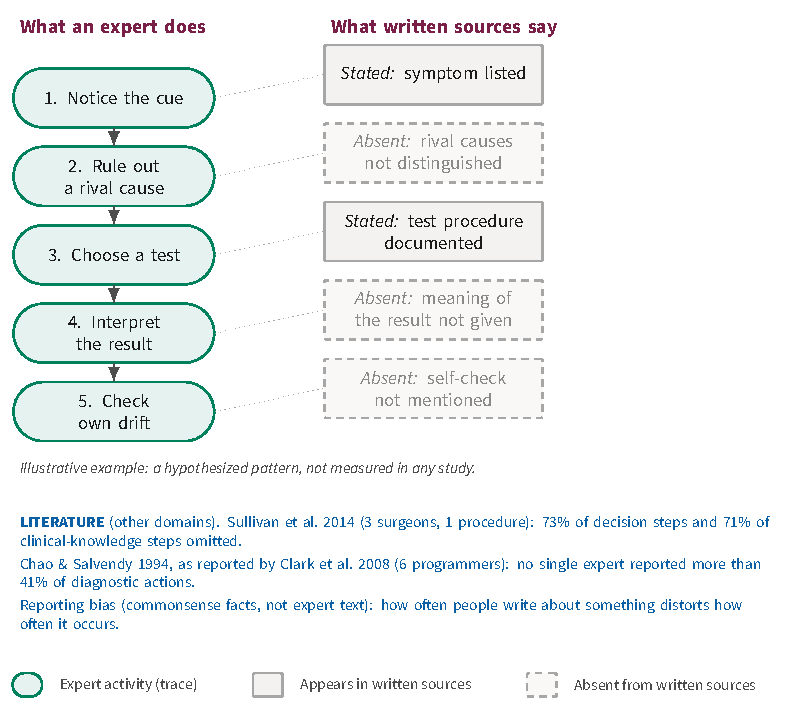
\includegraphics{figures/pdf/fig01_problem.pdf}
  \caption[What reaches text, and what does not]{What part of expert knowledge reaches text, and
    what does not. The task trace is illustrative, not measured. Automaticity and measured omission in
    three small studies show that experts' own reports leave out many decisions, cues and
    interpretations; reporting bias is shown for commonsense facts. That written expert sources omit
    the same kinds of knowledge is our hypothesis, not a finding of these studies.}
  \label{fig:problem}
\end{figure}

\subsection{Writers omit the obvious too}

\evlit{} How often people write about actions, outcomes and properties systematically distorts how
often they occur \parencite{gordon2013reporting}. Text-only language models inherit the distortion,
for example in the colors they predict for 521 objects \parencite{paik2021world}. Both studies concern
commonsense facts, not expert documentation. \evhyp{} We transfer the idea: omission in speech and
reporting bias in text may point at the same target in expert sources, namely cues, decisions,
interpretations, checks and the boundaries of hedged rules. This transfer is untested. AI can make the boundary between what is written and what is not sharper and more
auditable; it cannot tell on its own whether a silence hides expert knowledge, an unrecorded fact, or
nothing. That needs a human answer (\cref{fig:problem}).

\subsection{One education and one organizational example}

\evlit{} \emph{Education.} Experts sort physics problems by the principle that solves them; novices
sort them by surface features \parencite{chi1981categorization}. For the expert, choosing the
principle happens as recognition, not as a step, so it goes unsaid. Experts are also unreliable
judges of what learners find hard: 25 physics teaching assistants and 30 instructors predicted
students' most common wrong answers at 65\% and 68\% of the maximum score, against 40\% for random
guessing, with no difference between the groups \parencite{maries2016teaching}. Hence expert or AI guesses about
learner difficulty are never treated as evidence here.

\evlit{} \emph{Organizations.} Photocopier technicians diagnose through shared stories of how a
machine actually fails; those stories, not the service manual, keep the group's knowledge current
\parencite{orr1996talking,brown1991organizational}. \evobs{} On public PLC troubleshooting text, the
gap map produced a record of the same shape from the span \enquote{a common mistake\dots\ is
panicking and abandoning systematic approaches}: the sources name the failure mode, and the absence
check found at most a partial statement of how a troubleshooter notices the drift into
it.\footnote{\repo{research/n3/plc/gapmap.json}, the GUARD-lens record at rank~9.} This shows only
that a lens can flag text of this \emph{shape}.

\evlit{} \emph{Why it matters.} In a study of best-practice transfer inside firms, the major barriers
were knowledge-related (the recipient's lack of absorptive capacity, causal ambiguity, and an arduous
relationship between source and recipient) rather than mainly motivational
\parencite{szulanski1996exploring}. Many popular open-source projects depend on one or two developers
\parencite{avelino2016novel}, and turnover exposes projects to knowledge losses far above the expected
loss \parencite{rigby2016quantifying}. \evint{} Training, onboarding and succession can suffer when such
knowledge is not made explicit before its holder leaves.

\section{Question and hypotheses}\label{sec:question}

\begin{keyquestionbox}
  \textbf{RQ-B.} Can AI reconstruct what is written about a domain, and predict where its own
  reconstruction is thin, so that the location of the human knowledge residual is identified before
  any human is asked?
\end{keyquestionbox}

\textbf{H1 --- Reconstruction with provenance is feasible and checkable.} A system extracts atomic
claims from public sources, ties every evidence item to the exact span it came from, and labels each
claim's evidence status. H1 has an adversarial part: gating lets fewer planted falsehoods and false answers through
than the ungated model.

\textbf{H2 --- Lenses plus an absence check predict where experts add unwritten knowledge, by a margin
that matters.} Constructs from CTA and related methods, applied as lenses and followed by a check of
whether the expected element is stated, rank areas by where a fixed elicitation protocol brings out
validated knowledge the evidence lacks. Their area-level AUROC exceeds that of the strongest baseline
without this machinery, such as text density or a plain language-model guess, by at least $\delta$, a
smallest effect size of interest (SESOI). A real but smaller gain does not satisfy H2. \emph{H2 is the
central hypothesis.}

\begin{evfutbox}[unbreakable]
  \textbf{The falsifier.} $\Delta$AUROC is the gap map's area-level AUROC for ranking areas where the
  protocol elicits residual knowledge above the others, minus that of the strongest pre-registered
  baseline. H2 is falsified if the upper bound of a 90\% confidence interval on $\Delta$AUROC falls
  below $\delta$, fixed before any gold is acquired. H2 survives if the lower bound exceeds 0 and the
  point estimate reaches $\delta$; that rejects \enquote{no gain} but does not establish a gain of at
  least $\delta$, which only a lower bound above $\delta$ would. $\delta = 0.05$ is a provisional program
  threshold (\cref{sec:validation}). The blind prospective study (V5) reads this rule. It has not run.
\end{evfutbox}

\textbf{H3 --- Prioritized questions reduce expert time.} Questions chosen from the gap map recover
more validated, previously unwritten items per expert hour than an untargeted interview of equal length,
by a ratio of at least 1.25 (H3's SESOI, fixed before data); V6 reads it with the same rule form as H2.

\evint{} H2 means something only if H1 holds, and H3 only if H2's ranking beats chance.
\evhyp{} A separate hypothesis sits outside this chain. \textbf{H-OSS:} the gap map, adapted to code
and commit evidence, predicts where knowledge is lost when developers leave. It concerns
organizational artifacts, not the human residual, so it can neither support nor refute H2.


\begin{table}[htbp]
  \centering\small
  \caption{What the zero-participant PoC could test for each hypothesis, and its status. No cell
    reports a result against human knowledge.}
  \label{tab:hyp-status}
  \begin{tabularx}{\linewidth}{@{}p{0.05\linewidth}>{\raggedright\arraybackslash}p{0.3\linewidth}
      >{\raggedright\arraybackslash}X@{}}
    \toprule
    Hyp. & What the PoC could test & Status after the PoC \\
    \midrule
    H1 & Whether a ledger with verbatim provenance and cross-model verification runs end to end
      on real sources &
      \evobs\ Engineering part: yes for the pre-fix pipeline on PLC v1 and GDPR v1; the fixed pipeline has not completed a live run. Adversarial part: N2's registered verdict is INCONCLUSIVE; the
      gated arms were never scored (\cref{sec:results-n2}). \\
    H2 & Whether lenses fire on real text and the absence check separates \enquote{unstated} from
      \enquote{stated elsewhere} &
      \evobs\ Mechanism only. Lenses fire on three ledgers; the absence check ties its
      mismatched-evidence control.
      No $\Delta$AUROC computed. Next test: V1, before any grant. \\
    H3 & Whether ranked questions can be produced at all &
      \evfut\ Not tested. Template questions exist; no expert has answered one. \\
    \bottomrule
  \end{tabularx}
\end{table}

\section{From existing methods to the approach}\label{sec:approach}

Several research traditions each solve part of the problem. None answers the question this project
asks: \emph{in this domain, where does the written record stop, and what kind of knowledge is likely
to lie beyond it?} This section first states the approach, then what each tradition contributes to
it, then the closest prior work.

\subsection{The central model}\label{sec:approach-model}

\Cref{fig:model} shows the approach. Steps 1--6 are built in the PoC; steps 7--9 are not.

\begin{figure}[tbp]
  \centering
  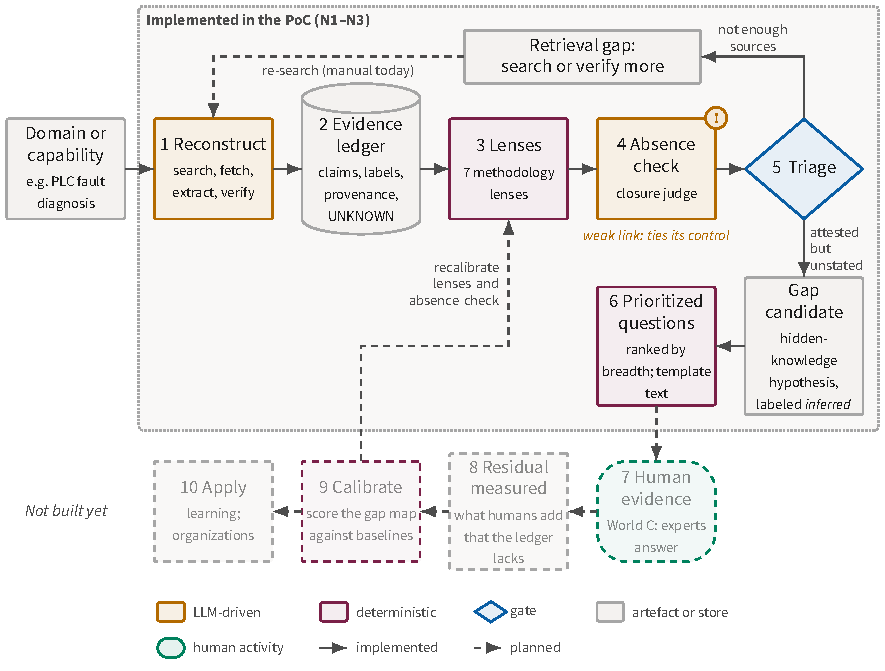
\includegraphics{figures/pdf/fig02_model.pdf}
  \caption[The central model]{What is the whole approach, and which parts exist today? Steps 1--6
    (solid) are implemented in the PoC; steps 7--9 (dashed) are future work. Triage splits the output
    into retrieval gaps, listed for further search, and gap candidates, which become hypotheses
    labeled \emph{inferred} and expert questions. The absence check (step~4) is the weak link.}
  \label{fig:model}
\end{figure}

\begin{description}[style=nextline, leftmargin=1.5em, itemsep=1pt, topsep=2pt]
  \item[1--2 Reconstruct into an evidence ledger] Fetch public sources, extract claims, locate each
    quote in a hashed snapshot, and verify it with a model of another family. Each claim carries one
    of six epistemic labels; \code{unknown} marks a slot searched and not covered.
  \item[3 Lenses] Seven lenses \emph{fire} when sources attest a construct but not its content, for
    example rival causes with no sign that separates them.
  \item[4 Absence check] A judge reads the sentences a lexical retriever pulls from the ledger (up to
    8 verified and 4 unverified per probe) and returns \emph{closed}, \emph{partial} or \emph{open};
    closed firings are dropped.
  \item[5 Triage] A \textbf{retrieval gap} (nothing found, one independent source, unverified text
    only, answered by a sibling run, or an unreadable verdict) calls for more search, not an expert.
    A \textbf{gap candidate} has at least two independent sources and an element the absence check
    did not find fully stated. It becomes a hidden-knowledge hypothesis labeled \code{inferred}.
  \item[6 Questions] Template-filled (no model writes them), with a predicted knowledge type and a
    human channel; ranked by a breadth rubric, not by expected information gain.
  \item[7--9 Future] Expert answers measure the residual, score and recalibrate the gap map, and only
    then feed instruction or organizational uses.
\end{description}
\evhyp{} If a lens fires, a working absence check does not find the missing element, and the attested
side has broad support, then practitioners are more likely there than elsewhere to hold knowledge the
text lacks. The PoC builds the mechanism; it does not test this hypothesis.


\subsection{What each tradition contributes}\label{sec:traditions}

\Cref{fig:lenses} shows which research tradition gives which lens, the missing element each lens looks
for, and the human channel that would ask about it. \evlit{} The traditions differ in strength. That
experts omit decisions, cues and interpretations is established in direction, from small studies in
single domains (\cref{sec:problem}). CTA-based instruction beats other ways of choosing training
content in a meta-analysis of few studies ($g = 0.871$; \cite{tofelgrehl2013cognitive}). The Critical
Decision Method, PARI, Evidence-Centered Design and knowledge components are established methods
\parencite{klein1989critical,hall1995procedural,mislevy2003structure,koedinger2012knowledge}. Causal
ambiguity rests on one large study of 271 observations \parencite{szulanski1996exploring}; the tacit
knowledge typology is conceptual, not empirical \parencite{polanyi1966tacit,collins2010tacit}; and
reporting bias is shown for commonsense facts, not measured in expert text
\parencite{gordon2013reporting}. \evint{} The literature therefore supports the \emph{constructs} the
lenses use. It does not support the lenses: no cited study tests whether a detector built on these
constructs finds real expert knowledge in text (Extended Technical Report, Section~3). Every mapping from
a construct to a lens is our interpretation, and every lens output carries the label \code{inferred}.

\begin{figure}[tbp]
  \centering
  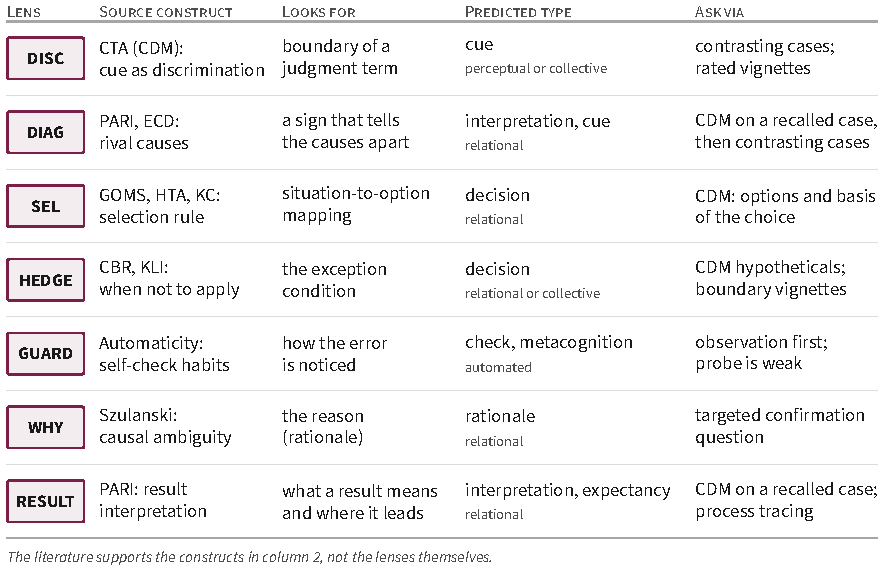
\includegraphics{figures/pdf/fig03_lenses.pdf}
  \caption[Which methodology gives which lens]{Which research method gives which methodology lens,
    what missing element each lens looks for, its predicted knowledge type, and the human channel
    that would ask about it. None of the lenses has been validated against a human judgment of where
    expert knowledge is missing.}
  \label{fig:lenses}
\end{figure}

\subsection{Closest prior work, and what may be new}\label{sec:novelty}

\evlit{} Our search, to September 2026, found precedent for every step. \textcite{torre2020ai} check
GDPR privacy policies for content types that a conceptual model of the regulation requires; on 24
unseen policies they found 45 of 47 incompleteness issues. That is typed absence detection in one of
our own domains, but the reference fixes in advance what should be present.
\textcite{anthonio2022clarifying} find underspecified phrases in instructional text, with later human
edits as gold. DRMiner mines design rationale from issue trackers \parencite{zhao2024drminer}.
\textcite{luitel2024improving} flag terms missing from requirements, and OntoAgent picks interview
questions from an ontology \parencite{jin2026chat}. \evint{} Each works on one document or interview
against a reference that already contains the missing content. None predicts what practitioners know
beyond all written sources, or routes a gap to an elicitation channel. \Cref{tab:novelty} places the
main elements.

\begin{table}[htbp]
  \centering\footnotesize
  \caption[Novelty ledger]{Condensed novelty ledger; the full ledger is in the Extended Technical Report, Section~4.3. \emph{Adaptation}: a known
    idea on a new unit or purpose.}
  \label{tab:novelty}
  \begin{tabularx}{\linewidth}{@{}>{\raggedright\arraybackslash}p{0.34\linewidth}
      >{\raggedright\arraybackslash}p{0.2\linewidth}>{\raggedright\arraybackslash}X@{}}
    \toprule
    Element & Category & Precedent or reason \\
    \midrule
    Claim ledger: verbatim spans from hashed snapshots, verifier of another family & Known
      combination & \textcite{min2023factscore,rashkin2023measuring} \\
    \code{unknown} only for a searched, uncovered slot & Adaptation & Abstention and completeness
      \parencite{razniewski2024completeness} \\
    Methodology lenses as absence detectors & Adaptation & Typed absence detection exists
      \parencite{torre2020ai,anthonio2022clarifying}; new here only the source of the types and the
      target. Validity not shown \\
    Knowledge type and elicitation channel per candidate & Adaptation / known method & Taxonomies and
      channel choice exist \parencite{collins2010tacit,klein1989critical} \\
    Retrieval gaps routed to search, not to experts & Adaptation & Retrieve-or-ask split in
      \textcite{taranukhin2026infogatherer} \\
    Synthetic output as predictor only, never criterion & Known method & Limits of simulated samples
      \parencite{bisbee2024synthetic} \\
    Scoring a gap map against published CTA results & Potentially novel (uncertain) & No such
      comparison found; gold sets are small \\
    Whole chain, domain-neutral, evidence status carried end to end & Potentially novel (uncertain) &
      No single system found; commercial tools may not publish methods \\
    \bottomrule
  \end{tabularx}
\end{table}

\evint{} The most defensible claim is the combination: a provenance ledger with an evidence status
per claim, expertise constructs as typed absence detectors, a knowledge type and channel per
suspected gap, and search failures kept apart from expert questions. It holds only as a proof of
concept. The evaluation design that scores a gap map against published CTA results is a stronger
novelty candidate than the system, but it has not run.

\section{What was built}\label{sec:built}

The PoC had one narrow engineering goal: a working, checkable chain from a named task to ranked
questions for an expert, using only public evidence and zero participants. It was built inside the
NOW program, which allows no participants, no proprietary data and no live interviews; its one human
input, a blind second coder, has not yet been used. \evint{} The constraint came from the project's
history. An earlier physics study, now frozen as Validation Track~A, built a complete, tested
instrument, but every one of its gates needed recruited physicists or students before any result
could be read (Extended Technical Report, Section~5).

\subsection{Architecture}

\evobs{} The PoC is three Python packages in a strict one-way dependency chain, checked by an
architecture test: \repo{residual/} (268 tests), \repo{reconstruct/} (416) and \repo{gapmap/} (172),
all offline with fakes, never a live model (Extended Technical Report, Section~6).
\repo{residual/} defines the typed evidence model.
\repo{reconstruct/} populates a ledger for one (domain, task) pair from the open web, in one
strictly ordered call with no agent loop: plan 3--6 areas with queries; search; fetch, normalize and
hash each document once into a content-addressed store; extract candidate claims; \emph{locate} each
quote verbatim in the normalized text (or produce no evidence at all); cluster documents into
independent sources; and \emph{verify} support with a model of another family. \repo{gapmap/} reads
one ledger and proposes gap candidates; it never writes a hypothesis back as a claim.


\evobs{} Planner and extractor are \code{anthropic/claude-haiku-4.5}; the verifier is
\code{openai/gpt-5.4-mini}. The code refuses a verifier from the extractor's family, so no claim gains
a criterion label by self-verification. The closure judge is \code{qwen2.5:7b-instruct}, run locally
at zero cost and chosen because its family differs from both. Its verdicts are cached by prompt hash,
so the gap map replays offline and byte-identically; only an explicit flag calls the model. A budget
check stops before overspending and writes the outputs as incomplete rather than truncating silently.

\subsection{The evidence model}

\evobs{} The atomic unit is the \code{ClaimRecord}. Each claim carries exactly one of six epistemic
labels (\cref{tab:labels}). The label is a computed property, never a stored field: nothing in the code
can set it by hand. A derived claim takes the weakest label among its premises, so a chain of
reasoning cannot bootstrap a strong label from a weak one. The evidential gate refuses any
\code{synthetic_extrapolation} input, and anything else outside the three criterion labels, before the
gated function runs. This is the code form of the project's central rule: \textbf{synthetic output may
be a predictor, never a criterion.}

\begin{table}[htbp]
  \centering\small
  \caption{The six epistemic labels (exact enum values). Only the first three can act as a
    criterion.}
  \label{tab:labels}
  \begin{tabularx}{\linewidth}{@{}lXc@{}}
    \toprule
    Label & Meaning & Criterion \\
    \midrule
    \code{observed_human_evidence} & Supported by a human-record (World~C) source & Yes \\
    \code{literature_supported} & Supported by a verified span in a public (World~A) source & Yes \\
    \code{organisational_artefact_supported} & Supported by a verified span in an organization's own
      (World~B) artifact & Yes \\
    \code{inferred} & Derived from other claims, with no direct support & No \\
    \code{synthetic_extrapolation} & Produced or supported only by a model & No \\
    \code{unknown} & Searched, fetched and fully examined by another model family; nothing found &
      No \\
    \bottomrule
  \end{tabularx}
\end{table}

\paragraph{Provenance.} \evobs{} Every fetched document is normalized once and hashed. A selector names
an exact character span inside that hash, and its text is the literal slice of the snapshot, never the
model's own quotation. The chain is \emph{snapshot hash $\rightarrow$ re-sliced span $\rightarrow$
claim}, so every evidence item can be re-checked offline with no model call. A claim whose quote cannot
be located gets no evidence and stays in the ledger under \code{synthetic_extrapolation}; it is not
dropped. Memorized model content can therefore enter the ledger, but only under a label no lens or gate
reads.

\paragraph{UNKNOWN, independence and contradictions.} \evobs{} A claim with no evidence enters under
\code{unknown} only when its slot was searched, fetched and fully verified with nothing found. Weaker
states (one source, unverified, never fetched) are tracked separately, because a slot never searched is
a retrieval failure, not a silence of the domain. Corroboration counts independent source clusters, not
documents. When two claims from different clusters conflict, the ledger stores a contradiction record
rather than merging them.

\paragraph{Evidence worlds.} \evobs{} Public (World~A), organizational (World~B) and human (World~C)
evidence are a typed field on each source, with validators. \textbf{Only World~A is populated in the
PoC}: World~B has no ingestion adapter and World~C has no data. The schema, the gap-map feature set and
the label code are hash-frozen together; a change needs a deliberate re-freeze and a commit saying why.

\subsection{N0--N3 and the verdicts they read}

\evobs{} Every NOW item is pre-registered to end in a continue, change or stop reading of an
experiment, never in \enquote{the build finished}.
\begin{itemize}[nosep]
  \item \textbf{N0} (reset; DOI hook, Track~A frozen): done, gate passed.
  \item \textbf{N1} (evidence model): done, gate \emph{continue with 2 additions}, at the registered
    limit of two.
  \item \textbf{N2} (reconstruction): engineering complete; registered research verdict
    \textbf{INCONCLUSIVE} (\cref{sec:results-n2}).
  \item \textbf{N3} (gap map): pipeline complete; hidden-knowledge prediction \textbf{not demonstrated};
    its program gate ($\Delta$AUROC against gold) has not run.
\end{itemize}
\evint{} Under the plan's rules, N2's inconclusive verdict would have blocked N3. The owner made one
recorded exception and treated N2's engineering milestone as enough to start N3. That was a softened
gate, softened by the person whose program depends on it, and no one outside the project checked it.
The validation program therefore adds an external gate reader (\cref{sec:validation}).

\section{Results}\label{sec:results}

\subsection{N2: reconstruction on the live web}\label{sec:results-n2}

N2 ran three experiments. E-LIVE checks that the pipeline runs on the live web without fabricating
or mislabeling; it has no gold and no threshold. E-PLANT and E-ABST are pre-registered, gated
experiments that compare the gated pipeline with an ungated raw model.

\paragraph{E-LIVE.} \evobs{} Two domains ran with the same models: PLC intermittent-fault diagnosis
(technical, procedural) and GDPR data protection impact assessments (legal, normative). A post-fix PLC
rerun crashed on a PDF encoding defect (0 claims). \Cref{tab:elive} gives the completed
runs.\footnote{\repo{research/n2/e_live_report.md}, \S3 and \S5; recomputed from each run's
\code{sidecar.json} and \code{ledger.json}.}

\begin{table}[htbp]
  \centering\small
  \caption{E-LIVE per-run counts. \enquote{Unknown claims} are slots searched, fetched and fully
    verified with nothing found. GDPR v2 is defect-compromised: 140 of its 366 evidence items kept a
    pending verdict after silent verifier failures, so it is not admissible for N3.}
  \label{tab:elive}
  \begin{tabularx}{\linewidth}{@{}Xrrrrrr@{}}
    \toprule
    Run & Sources & Extracted & Located & Verified & Unknown claims & Cost \\
    \midrule
    PLC v1 & 35 & 370 & 337 & 321 & 5 & \$0.679 \\
    GDPR v1 & 20 & 259 & 204 & 195 & 14 & \$0.500 \\
    GDPR v2 (not admissible) & 25 & 523 & 351 & 207 & 15 & \$1.002 \\
    \bottomrule
  \end{tabularx}
\end{table}

\evobs{} \emph{Exact spans.} All 909 evidence items of the three ledgers re-slice exactly from their
snapshots (337 + 206 + 366); a separate sample of 71 re-sliced 71 of 71, checked by an AI inspector,
not a human. The claims are a different matter: of 1,169 claims, 418 are labeled
\code{synthetic_extrapolation} (49, 64 and 305) and 34 \code{unknown}, so 452 (39\%) have no supporting
span. \emph{Verifier error.} On sampled claims the verifier's main error is scope drift, not
fabrication: 30\% on PLC v1 (Wilson 95\% CI 15--52\%, $n = 20$) and 12\% on GDPR v2 (4--30\%,
$n = 25$, in-sample). GDPR v1's 14 unknown slots concentrate in \code{failure_mode} (5 of 5 areas):
regulator text states obligations, not how an assessment goes wrong in practice; \evint{} this fits the
kind of gap the gap map targets, but it is not validated.

\evobs{} \emph{Decoys.} Supported claims were mutated (negation, a changed number or scope) and checked
again against the original span. The verifier accepted 7 of 20 decoys on PLC v1 (35\%, 18--57\%) and 3
of 20 on GDPR v1 (15\%, 5--36\%). Three PLC scope decoys only dropped a conjunct, so the span still
entailed them; without them the rate is 4 of 17 (24\%, 10--47\%). \evint{} The label
\code{literature_supported}, which every lens reads, rests on a verifier that accepted between a quarter
and a third of mutated PLC claims. A false \enquote{supported} claim can seed a gap candidate.

\evobs{} \emph{Defects found live.} Running on the real web surfaced eleven defects that 416 passing
offline tests had missed, among them verifier failures hidden behind a \code{complete: true} flag
(Extended Technical Report, Appendix~D). None of the fixes was re-checked live, and the current cross-verify and decoy stages have
never run live.

\paragraph{E-PLANT and E-ABST.} E-PLANT gives the raw model a false planted value among about 12 real
pages that state the truth, and asks whether it repeats the plant. Its validity floor assumed the
ungated model would adopt plants on more than 60\% of targets, a figure taken from ClashEval
\parencite{wu2024clasheval}. That figure holds only for two models, with the planted document as the only
context, a condition E-PLANT did not reproduce. E-ABST asks the raw model real but private questions and
counts false answers where it should abstain.

\begin{evobsbox}[unbreakable]
  \textbf{N2's registered verdict: INCONCLUSIVE.} The ungated model adopted $a_U = 5$ of 24 plants
  (21\%, Wilson 9--40\%), below the registered validity floor of 8. By the pre-registered rule this
  closed the Continue route before any gated arm was scored; it is a result about the test's
  sensitivity, not about gating. In E-ABST the raw model answered only 5 of 24 private items and
  abstained on 19 (79\%), so the required 20-point margin was reachable only in a narrow corner. The
  gated arms were never scored. \textbf{No statement about whether gating reduces planted falsehoods or
  false answers is supported.}
\end{evobsbox}

\evobs{} \emph{Budget stop.} N2's total spend was about \$4.82 against a \$5 weekly key limit (E-LIVE
\$2.374, E-PLANT \$1.953, E-ABST \$0.495), while the three experiments' registered caps summed to about
\$21. The post-fix live re-check (E-LIVE v3) stopped at its first call on the provider's key limit.
The owner chose not to raise it. \evint{} Budget headroom is part of the design: limits must be checked
against the sum of caps before a run sequence starts, and a \enquote{beats the baseline} gate must be
calibrated on a pilot before it is registered.

\subsection{N3: the gap map}\label{sec:results-n3}

\paragraph{Lenses.} \evobs{} Seven lenses fire over criterion-labeled claims only. They read the
extractor's paraphrase of each claim, not the verbatim span, and three of them depend on knowledge types
the extractor assigned. Lens firing tracks domain texture as designed: DIAG fires only on PLC, the
diagnostic domain; DISC and HEDGE fire mainly on GDPR, the normative one (\cref{tab:firing}). This shows
that lenses distinguish texture, not that they find hidden knowledge.

\begin{table}[htbp]
  \centering\small
  \caption{Lens firing per ledger. \enquote{Promotional excluded} counts candidates dropped before
    judgment by a domain denylist tuned in-sample.}
  \label{tab:firing}
  \begin{tabularx}{\linewidth}{@{}lrXr@{}}
    \toprule
    Ledger & Fired & By lens & Promotional excluded \\
    \midrule
    PLC & 56 & WHY 24, RESULT 19, DIAG 9, SEL 2, DISC 1, GUARD 1 & 42 \\
    GDPR v1 & 51 & RESULT 21, DISC 13, WHY 8, HEDGE 5, SEL 4 & 8 \\
    GDPR v2 & 48 & DISC 14, SEL 11, RESULT 9, WHY 9, HEDGE 5 & 1 \\
    \bottomrule
  \end{tabularx}
\end{table}

\paragraph{The absence check.} A fired lens only shows that a construct is named. Deciding that its
content is really \emph{unsaid} is the absence check. The PoC tried two versions.

\evobs{} \emph{Lexical closure} scored a candidate closed if another claim shared enough word stems.
Against a null of 200 random-donor draws, the observed closure counts fall within or below the null's
5--95\% interval on every ledger: PLC 22 against a null mean of 33.48 (26--41), GDPR v1 11 against
12.735 (8--17), GDPR v2 11 against 8.08 (5--12). Lexical closure did no better than chance.

\evobs{} \emph{Semantic closure}, the final version, asks the local judge to decide from retrieved
sentences whether the missing element is \code{closed}, \code{partial} or \code{open}. The fair control
keeps the seed's own sentences in both arms and swaps only the other-source sentences for those of the
topically nearest candidate of the same lens. Counting \code{partial} as closed, the judge's rate is the
same in both arms: \textbf{PLC 0.889, GDPR v1 0.961, GDPR v2 0.958} ($n = 54, 51, 48$). Every tested
lens in every ledger is flagged \code{closure-uninformative} (\cref{fig:closure}).\footnote{Each
\code{research/n3/*/gapmap.json}, field \code{checks.mismatched_evidence_control}.}

\begin{figure}[tbp]
  \centering
  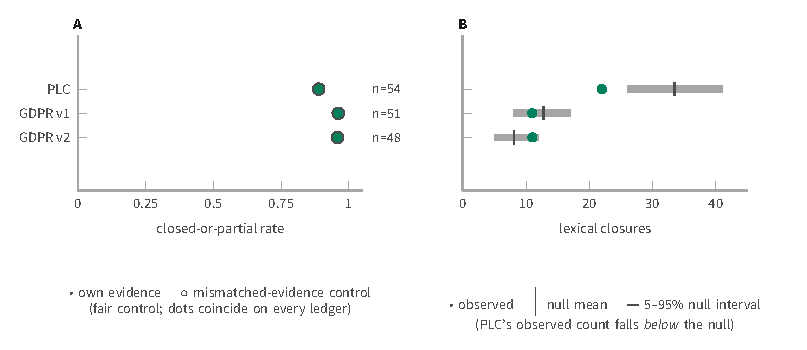
\includegraphics{figures/pdf/fig08_closure.pdf}
  \caption[The absence check versus its fair control]{Does the absence check beat its fair control?
    It does not. Panel~A: closed-or-partial rate on a candidate's own evidence and on the fair control,
    by ledger; the rates are equal. Panel~B: observed lexical closures against the donor null (mean and
    5--95\% interval of 200 draws).}
  \label{fig:closure}
\end{figure}

Four qualifications keep this in proportion. In 32 of the 153 pairs the two arms sent the judge an
identical prompt, so equality there holds by construction. Counted on \code{closed} alone, own versus
control is 0.30/0.33, 0.65/0.61 and 0.58/0.52, still far below the 0.20 difference the check requires.
The own rate is 1.0 on 11 of the 14 tested lens--ledger cells, so the test has little room. And an arm
with the seed's sentences removed still closes or partly closes 0.667, 0.725 and 0.708 of candidates,
which fits a lenient judge. \evint{} The reading is narrow: the judge's verdict does not depend on which
evidence it is shown. Every candidate reads \enquote{a lens fired here}, not \enquote{experts know
something here}. \evobs{} An adversarial AI review of the pre-final maps found this weakness; the first
built-in control had been a straw man that \enquote{passed}. The fair control now runs on every replay.

\needspace{5\baselineskip}
\paragraph{Triage, ranking and the display cap.} \evobs{} An unclosed firing becomes a retrieval gap
(\code{RG-UNK}: nothing found; \code{RG-SINGLE}: one independent source; \code{RG-UNVER}: closed only by
unverified text; \code{RG-SIBLING}: closed in a sibling run; \code{RG-UNDECIDED}: unreadable judge
answer), whose action is more search, or a gap candidate (\code{HYP}): an \code{open} or \code{partial}
record with at least two independent sources. A HYP record has three tiers: observed evidence, the
inferred gap, and a hypothesis whose label is fixed to \code{inferred}. Candidates are ranked by a
breadth rubric (independent sources, step breadth, penalties for \code{partial} and promotional seeds),
not by expected information gain. After merging near-duplicates, a display cap keeps at most 12 records,
3 per lens and 4 per area. On PLC it hides 15 of 24 merged candidates (10 RESULT, 5 WHY). Questions are
filled from fixed templates with up to two verbatim quotes; no model writes them.

\begin{table}[htbp]
  \centering\small
  \caption{Final map counts. GDPR v2 is shown only for the cross-run check. RG-UNK is a different
    quantity from N2's unknown claims (\cref{tab:elive}).}
  \label{tab:n3counts}
  \begin{tabularx}{\linewidth}{@{}>{\raggedright\arraybackslash}p{3.4cm}
      >{\raggedright\arraybackslash}X>{\raggedright\arraybackslash}X
      >{\raggedright\arraybackslash}X@{}}
    \toprule
    & PLC & GDPR v1 & GDPR v2 (not admissible) \\
    \midrule
    HYP after merge (uncapped) & 24: RESULT 13, WHY 8, DIAG 2, GUARD 1 & 1: RESULT &
      6: RESULT 3, DISC 1, HEDGE 1, WHY 1 \\
    HYP shown after the cap & 9: RESULT 3, WHY 3, DIAG 2, GUARD 1 & 1 & 6 \\
    Closure state of shown HYP & 3 open, 6 partial & 1 partial & 6 partial \\
    RG-SINGLE / UNVER / SIBLING / UNK & 11 / 0 / n/a / 10 & 12 / 4 / 2 / 28 & 3 / 6 / 7 / 44 \\
    \bottomrule
  \end{tabularx}
\end{table}

\begin{figure}[tbp]
  \centering
  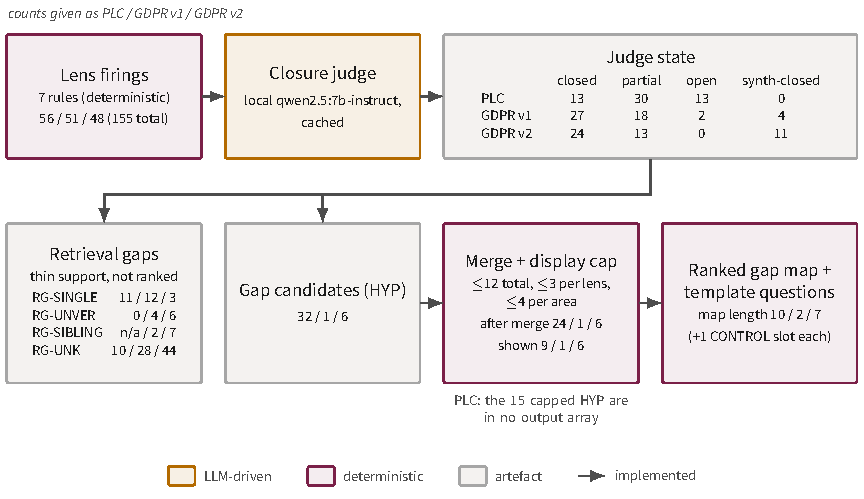
\includegraphics{figures/pdf/fig07_n3.pdf}
  \caption[From lens firing to gap candidate or nothing]{How lens firings become retrieval gaps, gap
    candidates or nothing, with counts per ledger (PLC / GDPR v1 / GDPR v2). After triage, near-duplicate
    HYP records are merged (PLC 24) and a display cap keeps at most 12 (PLC 9 shown). Most shown
    candidates are \code{partial}, not \code{open}.}
  \label{fig:n3}
\end{figure}

\needspace{6\baselineskip}
\paragraph{The negative results, stated plainly.}
\begin{itemize}[nosep]
  \item \evobs{} \textbf{13 of the 16 displayed candidates are \code{partial}.} The two PLC DIAG records
    read \code{open} only because the DIAG rule counts a partially signed rival cause as unsigned; only
    one displayed candidate (PLC rank~7, a WHY record) has no partial hit. \evint{} The fair control
    counts \code{partial} as closed, so most surviving hypotheses sit in a state the map's own control
    would call closed.
  \item \evobs{} \textbf{Precision by adversarial judgment: 3 of 19 strict (8 of 19 lenient), on the
    pre-final maps only} (Wilson 5.5--37.6\% and 23.1--63.7\%). One AI reviewer judged in-sample, with no
    human coder and no gold; the per-record tally is not committed, and the final maps were not
    re-tallied. It is a sanity signal, never a measured precision.
  \item \evobs{} \textbf{PLC's ranking follows source density} (Spearman $\rho = 0.91$; overlap of the
    top ten with the ten highest-density candidates $J_{10} = 0.58$). The anti-renaming check tests only
    the low-density direction ($J_{10} = 0.00$). On GDPR, $\rho$ is 0.09 and 0.16.
  \item \evobs{} \textbf{Cross-run stability is low.} Of GDPR v1's 13 unclosed lens records, 3 have a
    counterpart in the independent v2 run; of v2's 9, 3 have one in v1. Every counterpart is partial.
    \evint{} The runs are dominated by different sources, so the instability traces to retrieval.
  \item \evobs{} \textbf{A judge-parsing defect was found by review, not by tests.} Unparsed judge
    answers had silently defaulted to \code{open} (reported as 24 of 103, 62 of 150 and 60 of 147
    responses). The tests used a fake judge that always answered in format. Unparsable answers now
    become \code{RG-UNDECIDED}.
\end{itemize}

\subsection{One complete trace, and its weaknesses}\label{sec:trace}

\Cref{fig:trace} follows PLC's top-ranked record from source to question. The seed span, from a public
troubleshooting page, reads \enquote{Loose terminals cause many intermittent faults. A flashlight reveals
problems in dark panels that you miss otherwise.} The claim is \code{literature_supported}. Seven
independent sources discuss the topic, and the DIAG lens found five rival causes (ground loops,
aliasing, installation versus software, VFD/contactor noise, pull-up/clock timing). Of 34
verified sentences retrieved, the judge found none that fully states a sign separating any rival, and it
marked 5 claims as partial. The DIAG rule counts a partially signed rival as unsigned, so the record
reads \code{open}. The template question asks: \enquote{Which cause did you suspect first, and what did
you see, hear or measure that let you rule the others out?}, to be asked as CDM probes on a recalled
case, then contrasting cases.\footnote{\repo{research/n3/plc/gapmap.json}, \code{map[0]}, gap
\code{g-59164a9db5bd}.}

\evobs{} \emph{Weaknesses.} The trace was chosen by the author after the maps were final (the
top-ranked record of each map). The question's anchor is the extractor's assertion cut at 80
characters, so the question is not a grammatical sentence. The hypothesis template says the judge
\enquote{found a sign for the following} and then marks every item \enquote{(no sign found)}. The
\code{open} state overstates the evidence, since the judge found partial signs. PLC's second record
repeats the fragment defect, with rival causes such as \enquote{array subscript out of range.} Such a
candidate should not reach an interview unedited. \evint{} The trace shows that the mechanism runs from
a real span to a fixed-frame question, and where model-written text enters. It cannot show, without a
human answer, that the question would surface knowledge a practitioner holds.

\begin{figure}[p]
  \centering
  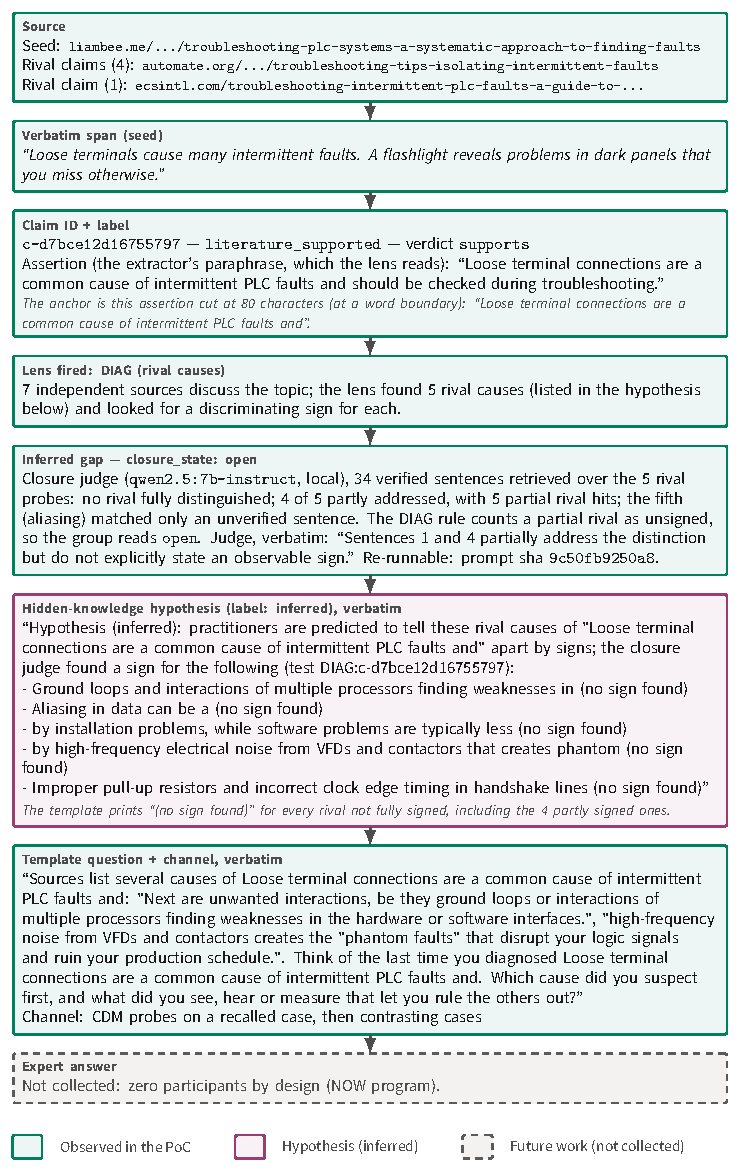
\includegraphics{figures/pdf/fig09_trace.pdf}
  \caption[One complete trace, source to question]{One complete real trace, end to end: seed span and
    claim, DIAG lens with five rival causes, the closure judge's verdict (no rival fully signed; 5 claims
    partly signed, counted as unsigned, so the record reads \code{open}), the hypothesis and the template
    question. The lens fired; the absence check found the element at most partly stated. No expert has
    answered the question.}
  \label{fig:trace}
\end{figure}

\section{What the PoC shows and does not show}\label{sec:shows}

\Cref{tab:shows} lists only what the repository artifacts support, and what they do not. The claims
are about the mechanism: that it runs, keeps its evidence traceable, and carries checks that expose
its own weakness. None is a claim about hidden expert knowledge. Evidence rows and artifact paths are
in the Extended Technical Report, Section~12 and Appendix~A.

\begin{table}[htbp]
  \centering\footnotesize
  \caption[What the PoC shows and does not show]{Part A: what the PoC demonstrates.
    \emph{Strong}: direct evidence checked by code or a test, or seen in more than one run.
    \emph{Moderate}: one run or in-sample. Part B: what it does not demonstrate, and what evidence
    would be needed.}
  \label{tab:shows}
  \newcommand{\nb}[1]{\multicolumn{2}{>{\raggedright\arraybackslash}p{\dimexpr0.52\linewidth+2\tabcolsep\relax}@{}}{#1}}
  \begin{tabularx}{\linewidth}{@{}>{\raggedright\arraybackslash}X
      >{\raggedright\arraybackslash}p{0.42\linewidth}>{\raggedright\arraybackslash}p{0.1\linewidth}@{}}
    \toprule
    \multicolumn{3}{@{}l}{\textbf{A. Demonstrated} \evobs} \\
    \midrule
    Claim & Main limitation & Strength \\
    \midrule
    The evidence model enforces its rules in code: computed labels, gates that refuse synthetic or
      unknown criteria, a hash-frozen schema & Tested offline; no World~B or C evidence has passed
      through & Strong \\
    Reconstruction runs end to end on live sources; every evidence item re-slices from its snapshot &
      One complete run per domain; 452 of 1,169 claims have no supporting span and are labeled so &
      Strong \\
    Cross-family verification and UNKNOWN slots operate & Operation, not accuracy: verifier error
      12--30\% by one AI inspector; cross-verify never ran live & Moderate \\
    Live runs expose defects offline tests miss, at small cost & Eleven fixes never re-checked live &
      Moderate \\
    The gap map runs end to end, keeps retrieval gaps apart from candidates, replays byte-identically &
      A display cap hides most PLC candidates & Strong \\
    The built-in checks expose the pipeline's main weakness & They show the absence check does not
      work yet, not that it can & Strong \\
    \midrule
    \multicolumn{3}{@{}l}{\textbf{B. Not demonstrated}} \\
    \midrule
    Claim & \nb{Why not, and what would be needed} \\
    \midrule
    That gap candidates are real tacit knowledge (H2) & \nb{No human has seen a candidate; no gold.
      Needs human-coded gold in held-out domains and a pre-registered test} \\
    That the absence check is informative & \nb{Ties its fair control everywhere. Needs agreeing human
      closure labels and a judge that beats the control (V1)} \\
    A precision for the gap map & \nb{Only one AI reading of pre-final maps. Needs two blind human coders
      on frozen maps} \\
    How many candidates the pipeline produces & \nb{Maps are capped; no area score. Needs a
      pre-registered area score over the uncapped set} \\
    Robustness to planted falsehoods; abstention & \nb{Gated arms never scored. Needs a calibration pilot,
      budget headroom, scored runs} \\
    Reconstruction quality against gold & \nb{\enquote{Supports} is a model's judgment; lenses read
      paraphrase. Needs expert-coded claims} \\
    Generalization and stability & \nb{Two domains, English web, in-sample tuning; two GDPR runs disagree.
      Needs held-out domains, a dated frozen corpus, repeated runs} \\
    That the ranking is not source density & \nb{$\rho = 0.91$ on PLC. Needs density and area size as
      headline baselines} \\
    Expected-information-gain question selection & \nb{Not implemented; ranking is a breadth rubric} \\
    Value for learners or organizations; World~B or C & \nb{Zero participants by design; typed fields
      only} \\
    
\bottomrule
  \end{tabularx}
\end{table}

\begin{findingbox}
  The PoC shows a working, checkable mechanism. It does not show that the mechanism finds real hidden
  knowledge. This report does not claim that the system identifies tacit knowledge, that the absence
  check found an element stated nowhere, that the ranking reflects real gaps rather than how much is
  written, that the pipeline resists planted falsehoods, that N2 passed or failed, or that every claim
  in the ledger is tied to a source span.
\end{findingbox}

\section{Interpretation and threats to validity}\label{sec:interpretation}

\begin{evintbox}
  The bottleneck is absence detection, not reconstruction and not lens firing. Reconstruction with
  provenance runs, and lenses fire in the expected places. What has no valid answer yet is \enquote{is
  this element really unsaid?} Every quantity after step~4 of the central model depends on it: which
  records become candidates, how they rank, which questions reach an expert, and any future score
  against gold. It must be validated against human closure labels before any gold test, or that test
  would score lens firing plus density, not the gap map.
\end{evintbox}

\evint{} Two features of the pipeline make the failure likely. Lenses fire on word stems in the
extractor's paraphrase, so they cannot see a paraphrase of the missing element and often fire where
the seed already states part of it. And most displayed candidates are \code{partial}: they mark places
where the text says \emph{something} about the element. Three caveats keep this from being a verdict on
absence detection as such: the judge is one small local model, a stronger judge is untested, and the
ceiling leaves little room for any difference.

\evint{} \textbf{Thinness is not the residual.} An area can be thin because the knowledge is unwritten,
or because retrieval was poor. \evobs{} The PoC ledgers show much of the second kind: in GDPR v1 one
independence key carries 194 of the ledger's key references and there are only three distinct keys; in
PLC v1, 11 of 35 fetched \enquote{sources} were error pages. \evint{} On PLC the ranking is close to
\enquote{how much is written about this topic}, which could look predictive for the wrong reason, since
experts may also have more to say about central topics. So density and area size must be headline
baselines, and the test must be conditional on them. The map is also partly a property of retrieval:
two runs of one task gave mostly different candidates. Any gold test needs a dated, frozen corpus and
repeated runs. Finally, lexicons, denylist and stop-anchors were tuned on the same ledgers, so any number
measured on them is optimistic; tuning did not rescue the absence check.

\begin{findingbox}
  The PoC neither demonstrates nor refutes H2. It does not demonstrate it: no gold, an absence check
  that ties its control, and a low, in-sample precision signal. It does not refute it: the registered
  stop rule needs held-out gold, a dated corpus, a frozen configuration, $\delta$, an area score and a
  second coder, and none exists. A negative result from a component not shown to measure its target
  says nothing about the target. The correct reading is \enquote{prediction not demonstrated, and the
  current absence check is not yet a valid instrument}, not \enquote{the human residual is
  unpredictable}.
\end{findingbox}

\begin{table}[tbp]
  \centering\footnotesize
  \caption{Main threats to the PoC's conclusions, what mitigates them now, and what the validation
    program does.}
  \label{tab:threats}
  \begin{tabularx}{\linewidth}{@{}>{\raggedright\arraybackslash}p{0.2\linewidth}
      >{\raggedright\arraybackslash}X>{\raggedright\arraybackslash}p{0.23\linewidth}
      >{\raggedright\arraybackslash}p{0.22\linewidth}@{}}
    \toprule
    Threat & Effect on our claims & Now & Program \\
    \midrule
    What a \enquote{gap} means & A firing plus an unclosed state may mark a paraphrase or a retrieval
      hole & Candidates labeled \emph{inferred}; retrieval gaps apart & Human closure labels (V1);
      gold tests \\
    Judge leniency, seed dominance, ceiling & Own rate 1.0 on most lenses; seed kept in both arms;
      the tie has several possible causes & Tie reported with closed-only, other-source-only and paired
      figures & Human labels in both arms (V1) \\
    Model paraphrase & Lenses and judge read the extractor's assertion, not the span & Spans kept
      beside every record & Lenses on spans; types checked in V1 \\
    In-sample tuning & Positive numbers would be optimistic & Configuration hashed; tuning disclosed &
      Hash-freeze before gold (MS2) \\
    Defaults that equal the finding & Unread answers became \enquote{open}; a first control could only
      pass & Parse fix; defects logged & Planted positives and nulls for every check \\
    Two domains, English web & Nothing generalizes beyond PLC and GDPR & Claims limited to these runs
      & Held-out domains after the freeze \\
    Non-reproducible retrieval & Web search, drifting pages and retiring models & Ledgers, snapshots,
      judge caches kept & Snapshot archives; dated corpora \\
    Tiny $n$, clustered units & Precision, verifier error, cross-run counts rest on 19--71 items that
      share sources & Wilson intervals (which assume independence) & Cluster-aware intervals; sizes set
      after pilots \\
    Single operator, owner incentive & One person designed, ran and read everything, and is the
      applicant & Committed artifacts; adversarial AI reviews & Non-owner blind coders; external gate
      reader \\
    AI-assisted development & Agent agreement can look like corroboration & Every number traced to an
      artifact & Human coders and pre-registration decide \\
    \bottomrule
  \end{tabularx}
\end{table}

\paragraph{What would change our mind.} \emph{Toward H2:} in blind prospective elicitation the lower
90\% bound of $\Delta$AUROC is above 0 and the point estimate at least $\delta$. \emph{Preconditions, not
evidence for H2:} coders agree on stated / partly stated / not stated ($\kappa \geq 0.70$) and a judge
beats the mismatched-evidence control and agrees with them; on pooled, dated, held-out CTA golds the
frozen map beats density, area size and a plain-LLM ranking, which shows compatibility with CTA-derived
representations. \emph{Against H2:} coders cannot agree whether an element is stated ($\kappa < 0.70$ after one
codebook revision); closure passes its human check yet the map adds nothing beyond density and area
size; or the prospective upper 90\% bound falls below $\delta$. \emph{Neither:} more runs on the same
ledgers, agreement among AI reviewers, or a stop reading from a configuration whose absence check never
passed its control.

\subsection{Threats to validity}

\Cref{tab:threats} lists the threats that could make the PoC's readings too strong or too weak (full
list: Extended Technical Report, Section~15).


\evint{} The PoC code, its adversarial reviews and this report were produced with AI agents under the
project lead's direction. The reviews found real defects, including the parsing defect and the failed
closure control, so they are useful as a search for errors. They cannot certify that errors are absent,
and they cannot serve as a criterion.

\section{The Human Knowledge Residual}\label{sec:residual}

The program has one target quantity that no one has measured: the Human Knowledge Residual (HKR).
\evint{} The term is not established. Its nearest analogues are unseen-item estimation
\parencite{chao1987estimating}, recall of knowledge bases \parencite{razniewski2024completeness} and
knowledge loss after developer turnover \parencite{rigby2016quantifying}.

\begin{evhypbox}
  Fix a task scope $D$ and an evidence base $E$: a set of sources found by a fixed search protocol and
  frozen at a date $t$. $\mathrm{HKR}(D, E, t)$ is the set of knowledge items that (1)~competent
  practitioners of $D$ \emph{demonstrably use}, corroborated by a second practitioner, a trace or an
  artifact outside $E$; and (2)~that $E$ \emph{does not contain}, as judged under a fixed codebook by
  blind coders or by a matcher that meets the adoption rule ($\kappa \geq 0.70$). We hypothesize that
  this set is not empty where practice matters, that it concentrates in cues, decision rules, checks and
  rationale, and that its location can be predicted from $E$ alone better than by cheap baselines.
\end{evhypbox}

The definition is relative: a new source can shrink the HKR. Let $R$ be what the reconstruction extracted and $H$ the validated human items. The observed residual share is
$|H \setminus R| \,/\, |H \cup R_{\mathrm{valid}}|$, reported per knowledge type and area. \evint{}
$H \setminus R$ is only an upper bound: it splits into the residual $H \setminus E$ and reconstruction
misses, items $E$ states that the pipeline did not extract. Telling them apart needs each item checked
against the frozen corpus, the \enquote{is it really unsaid?} decision the PoC's absence check did not
make reliably. So the residual cannot be measured more reliably than absence can be judged. An area is
\emph{residual-present} if it holds at least one validated, important item of $H \setminus E$; that is
the label the gap map is scored against.

\evint{} Three quantities must not be blurred. \emph{Thinness} is a property of the ledger alone; the
PoC computed it. The \emph{HKR} is a relation of $H$ to $E$; it is not yet measured. The \emph{gap-map
prediction} is an area score labeled \code{inferred}; none is built yet. Only the prospective study (V5)
measures the HKR as defined. The pooled CTA study (V2) uses published gold lists as a stand-in for $H$,
so it screens and does not decide. The departure study (V3) measures realized knowledge loss, a
different construct. \evobs{} The accounting types exist and refuse shortcuts: they raise an error when
an item lacks a human validity judgment and reject a matcher from the generator's family. No estimator
is implemented and no World~C data exist.

\section{The validation program}\label{sec:validation}

\evfut{} Nothing in this section has run; rules not yet registered are marked \enquote{proposed}.
The program asks for no money before its
cheapest decisive test has run, and each tranche is released only by a gate that reads CONTINUE. The
studies test one link at a time, and a failed link stops or reroutes everything above it: trustworthy
inputs (L0, V0), an informative absence check (L1, V1), retrospective prediction on published gold (L2,
V2), a measurable residual (L3, V4), prospective prediction (L4, V5, which decides H2) and practical
value (L5, V6--V8; V6 tests H3). \evint{} L1 comes first: with an uninformative closure step, a gold test
measures \enquote{a lens fired} plus density. The departure study V3 is off this chain; it tests H-OSS.

\begin{evfutbox}[float=tbp]
  \textbf{Gate rules, proposed for pre-registration.}\\[2pt]
  \textbf{MS1, closure verdict (end of Phase~0).} CONTINUE if human--human $\kappa \geq 0.70$ on the
  gating split (closed versus not closed), corpus-level retrieval recall meets its floor (proposed
  0.80), and at least one judge beats the fair control: its own-minus-control difference in the
  not-closed rate has a 95\% lower bound above 0 and lies within $\pm 0.10$ of the humans'. Otherwise STOP
  the automated absence check.\\[2pt]
  \textbf{MS3, screening gate for Phase~2 money (end of Phase~1).} CONTINUE only if the pooled
  retrospective $\Delta$AUROC has a point estimate $\geq \delta$, \emph{and} its lower 90\% bound is
  $> -\delta/2$, \emph{and} the map adds value over density and area size (conditional AUROC within
  density tertiles $\geq 0.5 + \delta$). Otherwise STOP H2 funding. MS3 is not a verdict on H2 and has no
  inconclusive route.\\[2pt]
  \textbf{MS5, H2 verdict (Phase~2).} STOP if the upper 90\% bound of the prospective $\Delta$AUROC is
  below $\delta$. CONTINUE if the lower 90\% bound is above 0 and the point estimate is at least
  $\delta$. Any other reading is reported as not supporting H2 and ends H2 funding.
\end{evfutbox}

\paragraph{Who reads the gates.} An external gate reader, an independent statistician or an advisory
board with one, reads MS1, MS3 and MS5 against the hash-committed pre-registration, with authority over
them. The reader is not a co-applicant and is not paid from a tranche the reading releases. Any owner
exception, at any gate, needs the reader's written sign-off, or the reading is void. \evobs{} No such
reader existed during the PoC, and none is named yet.

\subsection{Rules common to every study}

\evfut{} \emph{Two-step freeze.} The judge is chosen at MS1. Then MS2 (about month~4 of Phase~1)
hash-commits the pre-registrations, lexicons, thresholds, the adopted judge, the area score and the list
of eligible golds \parencite{nosek2018preregistration}. Only then is gold acquired and are held-out
domains reconstructed. \emph{Area score.} Every decisive test ranks areas, so Phase~1 builds a fixed
aggregation (for example the maximum or a noisy-OR) over the \emph{uncapped} candidates in each area,
chosen on pilot data only. \emph{Density.} Candidacy and rank are built from source counts, so a plain
gain over density is close to testing a variable against itself. The primary incremental analysis is the
area score's AUROC within density tertiles. \emph{Domains and dated corpora.} PLC and GDPR serve only for
debugging, V1 and an unanalyzed V5 pilot. Decisive studies use held-out domains on a corpus dated before
the criterion (archive captures and publications dated before the cutoff), with a per-gold blocklist and
a memorization probe on every model in the chain \parencite{golchin2023time,sainz2023nlp}.
\emph{Judges.} No LLM judge is a criterion. One is adopted only from another family than the generator,
with $\kappa \geq 0.70$ against blind human coders (the adoption rule), and re-checked on each new text
type before gold is unsealed; where it fails, closure there is human-coded.

\evfut{} \emph{Statistics.} Area-level AUROC is compared by DeLong's method or a cluster bootstrap
\parencite{delong1988comparing,obuchowski1997nonparametric}, with the strongest baseline chosen inside
each resample; MS5 has the logic of two one-sided tests \parencite{lakens2017equivalence}.
\emph{Choosing $\delta$.} Proposed $\delta = 0.05$: a smaller gain over density is unlikely to justify
reconstruction, while 0.10 would let a stop rule kill a real, modest gain. Under planning assumptions
without empirical basis (Hanley--McNeil errors, AUROC 0.70 against 0.62, error correlation 0.5;
\cite{hanley1982meaning}), the 90\% half-width of $\Delta$AUROC is about $\pm 0.14$ with 20 areas per
class, $\pm 0.10$ with 40, $\pm 0.06$ with 100 and $\pm 0.05$ with about 150.

\begin{figure}[tbp]
  \centering
  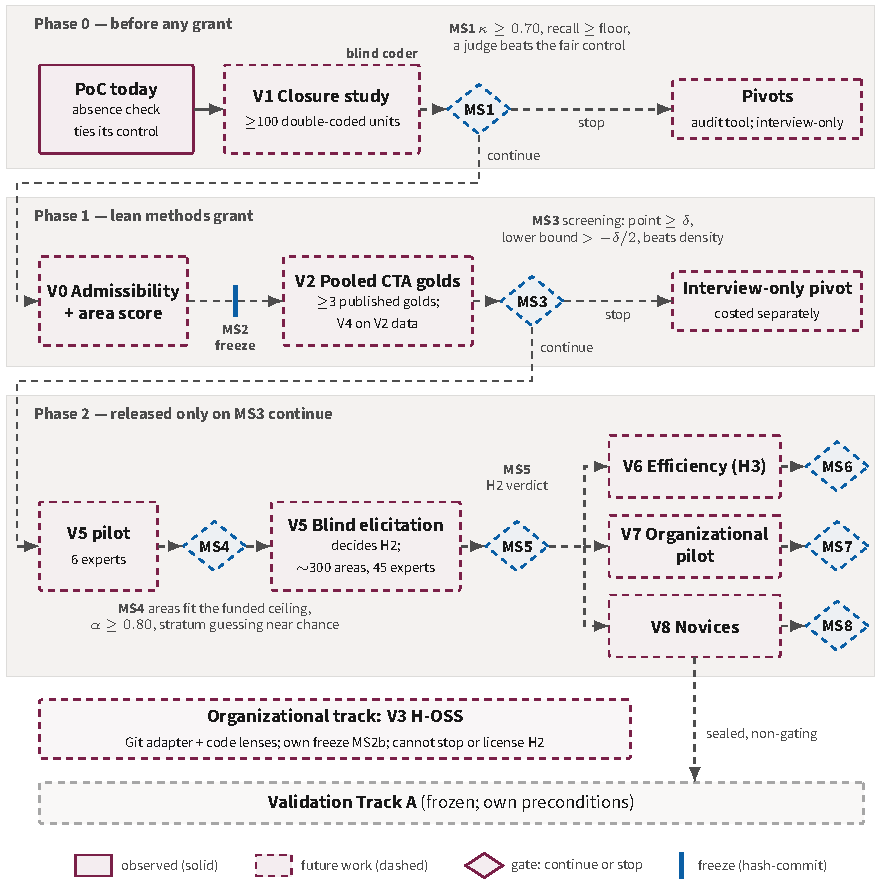
\includegraphics{figures/pdf/fig13_validation.pdf}
  \caption[The validation program]{Which studies, in which order, turn gap candidates into validated
    predictions, and which gate releases which money? Phase~0 (V1) ends at MS1. Phase~1 (V0, the MS2
    freeze, pooled V2, V4) ends at the MS3 screening gate. In Phase~2, V5 decides H2 at MS5 after its
    pilot gate MS4; only then do V6 (H3), V7 and V8 follow. V3 tests the separate hypothesis H-OSS.
    Stops lead to pivots. Track~A runs on a separate rail. All elements except the PoC are future work.}
  \label{fig:validation}
\end{figure}

\subsection{The studies}

Each study below is given by its design, people, measure, sample size and gate; the full protocols
and a per-study table are in the Extended Technical Report, Section~17.

\paragraph{Phase~0 --- V1, the closure study (before any grant).} \evfut{} \emph{Units:} a lens
firing with its seed span, missing element and evidence pool, in both arms of the fair control. All 107
admissible firings (PLC 56, GDPR v1 51) in both arms give 214 units; about 100 units from one new
non-gold domain are added so that no judge is scored only in-sample. \emph{Coders:} the judgment is
textual, so coders need codebook training, not domain expertise. The non-owner coder and the owner
(under origin blinding) code every unit, blind to arm, judge answer, rank and run. \emph{Retrieval
recall:} for about 50 firings the coder searches the ledger's full snapshots for the missing element.
\emph{Judges:} the local 7B model, a stronger open-weight model, and frontier models from other
families. \emph{Sample size:} with balanced classes, $\kappa \approx 0.70$ has a 95\% half-width of about
$\pm 0.10$ at 214 units. \emph{Cost:} tens of coder hours plus local compute, on the order of
EUR~$10^3$. \emph{On STOP:} pivot to reconstruction as a documentation-audit tool, or to interviewing
without a gap map.

\paragraph{Phase~1 --- V0, V2 and V4.} \evfut{} \emph{V0} makes pipeline outputs admissible as code,
builds the dated-corpus mode and the area score, and runs N2's deferred protocols after a calibration
pilot; its gate is the MS2 freeze (no hash, no gold). \emph{V2} scores the frozen gap map against
several published CTA task lists, pooled. A gold is eligible if it is an itemized list of steps,
decisions or cues from more than one expert, in a domain other than PLC, GDPR or Track~A physics, with
a dated corpus above a floor. Named candidates, in order: Sullivan's cricothyrotomy list, the only one
confirmed as itemized \parencite{sullivan2014use}; the NICU cue study \parencite{crandall1993critical};
the troubleshooting study \parencite{chao1994percentage}; and the PARI guide
\parencite{hall1995procedural}. Proposed: at least three golds, four to six if eligible. Each gold
domain is reconstructed once, from its dated corpus, before the sealed gold is acquired. Baselines
include random, area size, retrieval density, corpus frequency, a type prior from the other golds and a
plain-LLM ranking. \emph{What MS3 can read:} at four golds and 80 areas split evenly, the half-width is
about $\pm 0.10$, so CONTINUE needs a point estimate of at least 0.075. A map with no true gain passes
with probability about 0.11; a true gain of $\delta$ passes with about 0.34. \evint{} MS3 is a screen: it
accepts about a one-in-nine chance of releasing Phase~2 for a useless map, which V5 then stops. \emph{V4}
checks unseen-item estimators on V2 data against known truth; out of tolerance, only observed counts are
reported. It does not gate.

\paragraph{Phase~2 --- V5, blind prospective elicitation, which decides H2.} \evfut{} \emph{Design:}
freeze reconstruction, dated corpus, gap map, area score and partition. Sample areas in four labeled
strata: top of the area score (G), lowest retrieval density (D), top of a plain-LLM ranking (L) and
random (R). Each area gets a neutral CDM-style probe of about 8 minutes, the same for every area and
never the gap map's own question \parencite{klein1989critical}. \emph{Domains and people:} a PLC pilot,
not analyzed for effect; the main study in two held-out domains. Practitioners with several years of
practice, outside any Track~A pool, three per area \parencite{chao1994percentage}; one interviewer per
domain, two blind coders. \emph{Outcome:} an item counts if it is absent from the frozen reconstruction
\emph{and} the dated corpus, and is corroborated by a second expert, a trace or an outside artifact;
importance is rated blind to stratum. \emph{Blinding:} experts are told the study maps where practice
relies on unwritten knowledge, not that a model chose areas (partial disclosure, stated in the ethics
application, with debriefing). Interviewers see only area names in random order; a guess-the-stratum
check on 20\% of areas reports leakage. \emph{Sample size:} about 150 residual-present and 150 other
areas (300), 900 probes, about 45 experts at 20 areas each plus 6 in the pilot: about 150--250 expert
hours and 1,200--1,900 coder hours, roughly EUR~40--160k before staff time. \emph{Gates:} \textbf{MS4}
releases the main study only if the pilot (6 experts $\times$ 20 areas, 40 areas) projects at most 450
areas, segmentation reaches $\alpha \geq 0.80$, and stratum guessing stays near chance; otherwise V5 stops
and H2 is reported as untested prospectively. No underpowered V5 is ever run. \textbf{MS5} then reads its rule
in the gate box.

\paragraph{Phase~2 --- V6, V7, V8, only on MS5 CONTINUE.} \evfut{} \emph{V6 (H3, gate MS6)} is a
within-expert crossover of targeted questions against a standard unprompted-then-CDM interview; the
breadth ranking and selection by expected information gain (not built) are separate arms
\parencite{lindley1956measure}. Items first seeded by a question count only if independently
corroborated \parencite{loftus1975leading}. CONTINUE if the lower 90\% bound of the items-per-hour ratio
exceeds 1 and the point estimate is at least 1.25; STOP if the upper bound is below 1.25; any other reading
counts against H3. \emph{V7 (gate MS7)} is a descriptive pilot in one partner organization with 6--12
staff experts, after the deferred N2 validation; it goes multi-partner only if G areas beat D and R in
both parts. \emph{V8} covers the learner side: public learner data (no gate), 30--60 novices on confirmed
residual areas (MS8), and Track~A, touched only through sealed, secondary, non-gating predictions.

\paragraph{Organizational track --- V3 (H-OSS).} \evfut{} None of its components exists: a Git adapter
that turns commits, issues and reviews into claims with exact spans, areas mapped to code units at a
time before a departure, and lenses for code text, frozen at MS2b once the adapter exists. The outcome is
blind-coded rationale-seeking issues and defect-fix commits after truck-factor departures
\parencite{avelino2016novel}, analyzed as a staggered difference-in-differences
\parencite{callaway2021difference}, against baselines that include authorship concentration and knowledge
at risk \parencite{rigby2016quantifying}. A 5-departure pilot sizes the study; its gate uses the MS5 rule
on H-OSS only. It can neither stop nor license H2.


\evint{} Each STOP teaches something. At MS1 it shows that absence in text cannot yet be judged
reliably, and it leaves a public closure set. At MS3 it leaves a reconstruct-versus-CTA benchmark. At
MS5 it falsifies, with a bounded effect size, the claim that text reconstruction locates the human
residual. Program threats (incomplete gold, method-dependent elicitation, matcher error) are treated
there too.

\section{Platform and applications}\label{sec:platform}

\evfut{} The platform described here does not exist. The PoC is one walking skeleton toward it, and a
gap candidate remains a prediction until a human answers it.

\paragraph{Three evidence worlds.} Every piece of evidence belongs to one world, already a typed field
in the code. \emph{World~A}, public evidence (textbooks, papers, standards, forums, public learner
data), can yield concepts and taught heuristics, but not episode-specific cues or local practice.
\evobs{} It is implemented for open-web text only. \emph{World~B}, organization-specific evidence
(procedures, tickets, commits, reviews, logs, incident reports), adds a second axis, practice:
prescribed (\code{imagined}), recorded (\code{done}) or reported. \evhyp{} The gap between imagined and
done is the organizational form of the residual. \evobs{} The schema exists; no ingestion does.
\emph{World~C}, human evidence (elicitation, ratings, learner responses, coder labels), has types but no
data. \evfut{} A and B build the reconstruction; the gap map predicts where C is needed; C answers through
the channel matched to the predicted knowledge type and is the only path that can score the predictions.
C never edits the reconstruction in place, and at least one human arm stays blind to the reconstruction,
or anchoring shrinks the measured residual.

\paragraph{Rules the platform keeps.} \evobs{} Labels are computed, never set. A label is only as strong
as its weakest link. Derived outputs (gap records, scores, questions) are \code{inferred} at best, and the
evidential gate refuses them as a criterion. \evfut{} Labels move up only through World~C or
cross-family verification; World~B claims never leave their organization's tenant; and
\textbf{unvalidated candidates never reach a learner or an end user}. No code enforces these three yet.
On premises, the platform needs three model families available locally (generator, verifier, closure
judge). \evobs{} The PoC already runs its judge locally, which shows the pattern is viable and also its
risk: that 7B judge did not beat its fair control. Organizational deployment adds per-user access control
propagated to claims, retrieved text treated as data and never as instructions, and a hash-chained audit
trail (Extended Technical Report, Section~18).

\begin{figure}[tbp]
  \centering
  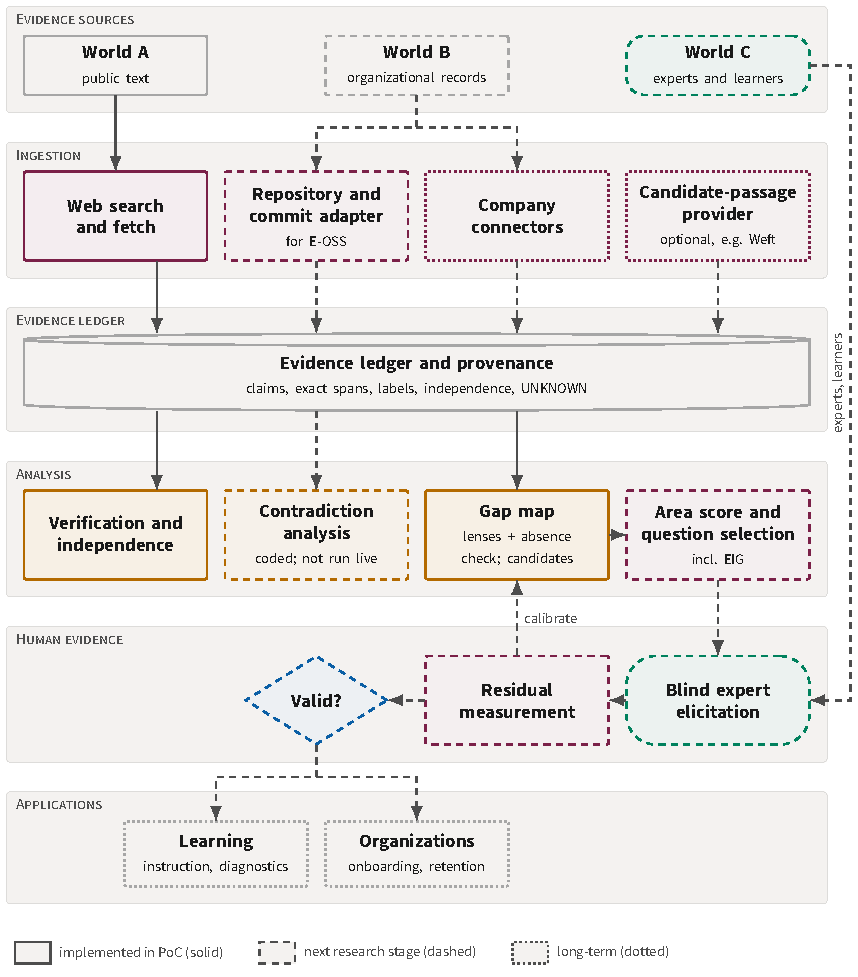
\includegraphics{figures/pdf/fig11_platform.pdf}
  \caption[Platform layers]{What would the full platform contain, and what exists today? Layers run from
    evidence sources through acquisition, provenance, the evidence ledger, analysis, the human loop and
    applications, with validation, audit and security as a rail. Solid boxes exist in the PoC; dashed
    boxes are the next research stage; dotted boxes are long-term. Only World~C evidence can score the gap
    map's predictions.}
  \label{fig:platform}
\end{figure}

\evobs{} What exists today is the evidence ledger with its frozen schema, provenance verification on open
web text, the gap map (candidates only), gates and checks, and a per-run call and cost log. Contradiction
analysis beyond the older pairwise stage, company retrieval, expert elicitation for new tracks, residual
measurement and expected-information-gain question selection are the next research stage; learner
diagnostics, instructional design and adaptive learning are long-term. \emph{Weft}, a separate public
retrieval engine, was assessed as a possible future World~B layer; it keeps no in-document character
offsets and no per-user access control, so integration is not justified now, and at most it could
supply candidate passages that the platform re-hashes and re-locates itself.

\subsection{Education}

\evlit{} Expert judgment of learner difficulty is unreliable (\cref{sec:problem}), so the education path
routes \enquote{what is difficult} through learner data alone. CTA-based instruction outperforms other
ways of identifying training content in a meta-analysis of a small number of studies ($g = 0.871$;
\cite{tofelgrehl2013cognitive}); in one biology course (N~=~314) CTA-derived instruction cut withdrawal
from 8.1\% to 1.4\% \parencite{feldon2010translating}. A worked example that prompts the learner to
generate a step beats one that states it ($g = 0.35$, $k = 6$; \cite{bisra2018selfexplanation}). But a
single item response is a poor diagnostic unit: 31\% of Force Concept Inventory answers changed on a
one-week retest \parencite{lasry2011fci}. A synthetic learner returns the misconception it was handed:
a GPT-4 simulation of that inventory showed no response variance until told which preconception to hold
\parencite{kieser2023chatgpt}. And the median effect in 747 randomized education trials was 0.10~SD
\parencite{kraft2020interpreting}.

\evint{} The pipeline is therefore evidence-complete only as far as \enquote{instructional material},
and only for items validated by humans. Synthetic learners serve only to pilot a probe or debug a
pipeline, never as evidence. A candidate education pilot would add one or two expert-confirmed operations
to self-explanation prompts in one course section and measure delayed transfer, as a feasibility pilot,
not a powered test. Validation Track~A (twelve physicists; about 370 students in a two-arm trial with
delayed transfer, futility test at $d = 0.30$) runs only on its own preconditions, with its registered
rules unchanged; this program touches it only through sealed, secondary, non-gating predictions.

\subsection{Organizations}

\evlit{} Three organizational blind spots have literature behind them: a technician's diagnostic cue,
carried in stories rather than manuals \parencite{orr1996talking}; a senior engineer's design rationale,
lost to causal ambiguity \parencite{szulanski1996exploring}; and a compliance officer's exception
judgment, the gap between work as imagined and work as done \parencite{hollnagel2018safety}. Turnover
loss is measurable in software: 65\% of 133 popular GitHub projects have a truck factor of 2 or fewer
\parencite{avelino2016novel}, and 315 of 1,932 projects (16\%) were abandoned after truck-factor
developers left \parencite{avelino2019abandonment}. \evobs{} The PoC produced candidates of the first and
third shape (the PLC GUARD record; a GDPR v2 record built on the \enquote{in most cases / in some cases}
hedge of the DPIA guidance), both unvalidated, the second from an inadmissible run.

\evhyp{} Every value proposition is untested: that a gap map shortens onboarding, turns into a capture
priority for a retiring expert, or adds predictive value beyond authorship concentration (which H-OSS
tests). We found no credible, peer-reviewed cost figure for organizational knowledge loss in general and
claim none. \evint{} The limits are hard ones. A World~B run needs access-scoped retrieval, on-premises
or contractually isolated models, re-tuned lexicons, and a data protection impact assessment; where a
German entity is involved, a works agreement. Outputs are aggregate by default, never feed performance
evaluation, and name a person only with consent. A coverage score used as a target would reward
documentation that raises the score over documentation that transfers knowledge. The recommended first
partner is a software organization, closest to the registered H-OSS design.

\section{Plan: domains, money, team and risks}\label{sec:plan}

\evfut{} Everything in this section is future work, and every figure is a planning range.

\subsection{Domains}

A domain is chosen for the generalization question it answers and the human criterion that can test it,
never for convenient data (\cref{tab:domains}). Three binding rules apply. Physics is the frozen Track~A
domain and enters only through sealed predictions. A held-out gold domain is never reconstructed before
its configuration is frozen: its first reconstruction \emph{is} the test run. PLC and GDPR tuned the
lexicons, so they never carry a gate reading. Hence the recommended design: a V5 pilot in PLC, not
analyzed for effect, and the V5 main study in a fresh maintenance-diagnosis task (D3) and a held-out
regulation (D4).

\begin{table}[htbp]
  \centering\footnotesize
  \caption{The six proposed domains. D1, D3 and D4 carry H2's gates; D2 carries H-OSS only; D5 and D6
    gate nothing for H2.}
  \label{tab:domains}
  \begin{tabularx}{\linewidth}{@{}>{\raggedright\arraybackslash}p{0.17\linewidth}
      >{\raggedright\arraybackslash}X>{\raggedright\arraybackslash}p{0.27\linewidth}
      >{\raggedright\arraybackslash}p{0.17\linewidth}@{}}
    \toprule
    Domain & Question & Criterion & Role \\
    \midrule
    D1 Clinical procedure & Does the map find omitted steps and cues in a decision-heavy procedure? &
      Pooled published CTA golds, Sullivan's 46-item list first & V2; MS3 screen \\
    D2 Open-source maintenance & Does artifact coverage predict realized knowledge loss? & Blind-coded
      trouble after truck-factor departures & V3 (H-OSS); V7 precursor \\
    D3 Industrial fault diagnosis & Does it hold where craft dominates and text is poor? & Prospective
      blind elicitation & V5; MS5 \\
    D4 Regulatory judgment & Does it work where the residual sits in hedges and exceptions? &
      Prospective blind elicitation & V5; MS5 \\
    D5 School mathematics & Does an expert-text residual relate to learner difficulty? & Public learner
      response data & Learner link only \\
    D6 Introductory mechanics & Best-case ceiling where residual, learner error and an RCT meet & Track~A's
      own registered rules & Secondary, non-gating \\
    \bottomrule
  \end{tabularx}
\end{table}

\subsection{Roadmap and the money each gate releases}

\Cref{fig:roadmap} shows the phases. Phase~0 runs alone and needs no grant, no participants and no new
software. Phase~1 builds nothing for Phase~2, so no Phase~2 spending runs ahead of MS3. \Cref{tab:money}
gives each tranche. Personnel is costed at EUR~6--10k per person-month, to be replaced by the host
institution's rate.

\begin{figure}[tbp]
  \centering
  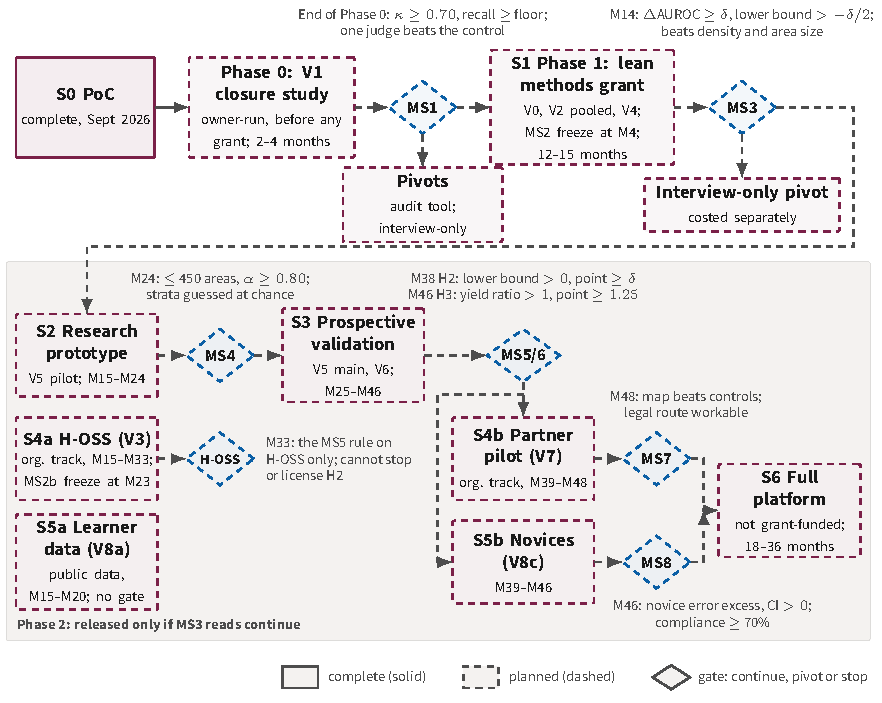
\includegraphics{figures/pdf/fig14_roadmap.pdf}
  \caption[Gated roadmap]{Which gated stages lead from PoC to platform? Phase~0 (owner-run, before any
    grant) is the closure study, ending at MS1. Phase~1, a lean methods grant, starts only on MS1
    CONTINUE and ends at the screening gate MS3. Phase~2 starts only on MS3 CONTINUE; its prospective
    study decides H2 at MS5. Every stop leads to a pivot with its own, smaller budget. Only S0, the PoC, is
    complete.}
  \label{fig:roadmap}
\end{figure}

\begin{table}[htbp]
  \centering\footnotesize
  \caption{Tranches, the gate that releases each, and indicative cost. Months count from the start of
    Phase~1.}
  \label{tab:money}
  \begin{tabularx}{\linewidth}{@{}>{\raggedright\arraybackslash}p{0.13\linewidth}
      >{\raggedright\arraybackslash}p{0.13\linewidth}>{\raggedright\arraybackslash}X
      >{\raggedright\arraybackslash}p{0.1\linewidth}r>{\raggedright\arraybackslash}p{0.13\linewidth}@{}}
    \toprule
    Tranche & Released by & Scope & Months & PM & Total (EUR) \\
    \midrule
    Phase~0 & Owner, no grant & V1 closure study & 2--4 mo before M1 & -- & $\approx 10^3$ \\
    Phase~1 & MS1 continue & Area score, freeze, V0, judge check, pooled V2, V4 & M1--M14 & 35--44 &
      \textbf{0.23--0.51\,M} \\
    2a & MS3 continue & Workbench, V5 pilot, learner data, ledger groundwork & M15--M24 & 29--44 &
      0.19--0.49\,M \\
    2b & MS4 continue & V5 main, powered & M25--M38 & 22--36 & 0.17--0.61\,M \\
    2c & MS5 continue & V6, V7, novice study, education pilot, on-prem stack & M39--M48 & 38--62 &
      0.26--0.79\,M \\
    O & MS3 continue & Git adapter, code lenses, V3 (H-OSS) & M15--M36 & 14--22 & 0.09--0.26\,M \\
    \midrule
    \textbf{Phase~2} & & 2a--2c and O & M15--M48 & 103--164 & \textbf{0.7--2.2\,M} \\
    \textbf{Program} & & Phases~1 and 2 & 48~mo & 138--208 & \textbf{0.9--2.7\,M} \\
    Interview-only pivot & MS1, MS3 or MS5 stop & Separate proposal & 18--24~mo & 21--31 & 0.14--0.38\,M
      \\
    \bottomrule
  \end{tabularx}
\end{table}

\evint{} \textbf{Money at risk if H2 fails}: at MS1, about EUR~$10^3$ plus the owner's time; at MS3,
Phase~1 (EUR~0.23--0.51\,M), which still leaves a released closure set, a frozen area score and a public
benchmark; at MS4, EUR~0.42--1.00\,M; at MS5, EUR~0.59--1.61\,M, and tranche 2c is never released. The
binding constraint of V5 is recruiting about 45 eligible experts, not money. \evobs{} The PoC's one hard
cost number: a reconstruction run cost \$0.50--\$1.00. Money was not the constraint; headroom was.
\evint{} So provider limits are set at least three times the sum of a stage's registered caps, the
headroom check runs as code, each experiment has its own key, and every study reports cost per
\emph{validated} item.

\subsection{Team}

\begin{evfutbox}
  \textbf{Team status.} No team exists yet: no host institution, no principal investigator (PI) record
  for this program, no statistician, no CTA collaborator, no gate reader and no letter of support. One
  operator designed, built, ran and read the PoC with AI assistance, and is the prospective applicant.
  Before MS1 is read: the non-owner blind coder and the external gate reader. Before the Phase~1
  proposal: host institution, PI, statistician as co-applicant, CTA collaborator, research engineer,
  data-protection and license advisor. Before Phase~2: a cognitive psychologist or CTA lead, expert
  pools with letters from professional bodies, and a learning scientist.
\end{evfutbox}

\evint{} The hard problems span language processing and measurement, CTA, learning science, statistics,
and security, privacy and law, so the team is interdisciplinary. It grows only when a gate releases the
next phase (\cref{tab:team}).

\begin{table}[htbp]
  \centering\footnotesize
  \caption{Team by phase. Phase~1 (12--15 months, about 2.5--3.0~FTE, 35--44 person-months) reaches
    MS3; Phase~2 (34 months, about 3.0--4.8~FTE on average across 6--8 people) is hired only on MS3
    CONTINUE. Full role tables: Extended Technical Report, Section~24 and Appendix~H.}
  \label{tab:team}
  \begin{tabularx}{\linewidth}{@{}>{\raggedright\arraybackslash}p{0.3\linewidth}
      >{\raggedright\arraybackslash}p{0.14\linewidth}>{\raggedright\arraybackslash}p{0.14\linewidth}
      >{\raggedright\arraybackslash}X@{}}
    \toprule
    Role & Phase~1 FTE & Phase~2 FTE & Main work \\
    \midrule
    PI / research lead & 0.8--1.0 & 0.5--1.0 & Hypotheses, thresholds, gate reports (never reads a
      gate) \\
    Research engineer (LLM / retrieval) & 1.0 & 0.5--1.0 & Area score, freeze, dated corpora; judge
      upkeep, on-prem models \\
    Research assistant or second engineer & 0.5 & -- & Gold availability, partitions, memorization
      probes \\
    Statistician / methodologist & 0.3 & 0.3--0.5 & Threshold table, pooled and clustered AUROC \\
    CTA practitioner / cognitive psychologist & 0.1--0.2 & 0.5 $\to$ 1.0 & Codebook, gold mapping; V5
      interviewing \\
    AI/ML researcher & -- & 1.0 & Prospective designs, baselines, repository mining \\
    Platform engineer & -- & 1.0 & Git adapter, workbench back end, audit trail \\
    Learning scientist; HCI; project manager; legal & -- & part-time & Learner link; leak-proof
      interfaces; partner contracts; DPIA \\
    Coders & 160--380\,h & 1,000--2,000\,h & Blind double coding \\
    External gate reader & per gate & per gate & Reads MS1, MS3, MS5; independent \\
    \bottomrule
  \end{tabularx}
\end{table}

\evint{} One staffing rule cannot be relaxed by adding people: an advisor who saw a domain's gap map may
not later be interviewed, code, rate or corroborate in that domain; the pipeline's owner is never the
only coder on a gating score; interviewers and coders never see scores or strata.

\subsection{Top risks and kill criteria}

\begin{table}[htbp]
  \centering\footnotesize
  \caption{Risks that can stop or redirect the program (likelihood / impact, qualitative). Full table:
    Extended Technical Report, Section~26.}
  \label{tab:risks}
  \begin{tabularx}{\linewidth}{@{}>{\raggedright\arraybackslash}p{0.22\linewidth}
      >{\raggedright\arraybackslash}p{0.05\linewidth}>{\raggedright\arraybackslash}X
      >{\raggedright\arraybackslash}p{0.33\linewidth}@{}}
    \toprule
    Risk & L/I & Early signal & Kill / pivot criterion \\
    \midrule
    Absence check cannot be made informative & H/H & \evobs{} Own rate equals control rate on every
      ledger & MS1 fails $\to$ stop the automated absence check; no grant for the gap map \\
    Gap map does not beat the strongest baseline & M/H & PLC ranking tracks density ($\rho = 0.91$) &
      MS3 fails $\to$ no Phase~2 money; MS5 short of CONTINUE $\to$ H2 not supported \\
    Too few golds & M/H & Fewer than three eligible itemized golds & MS3 rule unchanged, so CONTINUE
      gets harder; nothing stands in \\
    Contamination & H/M & Many probe-positive items & Drop that gold from the pooled reading \\
    Expert recruitment & M/H & Pilot projects more than 450 areas & MS4 $\to$ V5 main not released; H2
      untested \\
    Owner overrides a gate & M/H & An exception like N2 $\to$ N3 & Without reader sign-off the reading is
      void \\
    Team / key person & H/H & No host, no named team & Program pauses at its last gate \\
    Budget headroom & L--M/M & Limit below the sum of caps & Rerun with headroom; never read as
      negative \\
    Ethics / legal (V7) & M/H & DPIA risk or works-council objection & Stop the pilot at that partner \\
    \bottomrule
  \end{tabularx}
\end{table}

\evint{} Two pivots exist, each on its own budget. The \emph{interview-only pivot} compares question
selection by expected information gain with untargeted interviewing, without any reconstruction prior; a
negative result bounds how far text reconstruction can go. The \emph{documentation-audit pivot} keeps the
ledger as a provenance-checked map of what a text states, with no claim about hidden knowledge.

\subsection{Expected contributions}

\evobs{} Three contributions exist today, independent of H2: a provenance-typed evidence model,
self-checks built into every gap map, and documented negative and inconclusive results. The novelty
ledger grades them as known methods, known combinations or engineering. \evfut{} \Cref{tab:contrib} lists
what the program would add; every row delivers something even on a stop.

\begin{table}[htbp]
  \centering\footnotesize
  \caption{Expected contributions, graded by outcome. All rows are future work.}
  \label{tab:contrib}
  \begin{tabularx}{\linewidth}{@{}>{\raggedright\arraybackslash}p{0.25\linewidth}
      >{\raggedright\arraybackslash}X>{\raggedright\arraybackslash}X@{}}
    \toprule
    Contribution (study) & If it holds & Even if it fails \\
    \midrule
    Human-labeled closure set (V1) & \evhyp{} A validated way to judge \enquote{not stated in this
      evidence} & A measured answer to whether absence can be judged; a public benchmark \\
    Pooled CTA-gold benchmark (V2) & \evhyp{} A first retrospective $\Delta$AUROC, conditional on density
      & A contamination-controlled test for any system that claims to find what text omits \\
    Post-departure dataset (V3) & \evhyp{} Coverage predicts loss beyond authorship & Evidence that it
      does not; a public outcome set \\
    Residual corpus (V5) & \evhyp{} Calibration data for gap maps & A typed record of what experts add
      beyond a fixed text \\
    Efficiency (V6) & \evhyp{} At least 1.25 times more validated items per expert hour & A bound on the
      gain \\
    Learner link (V8) & \evhyp{} Residual areas carry more novice errors & Evidence that the two are
      different constructs \\
    \bottomrule
  \end{tabularx}
\end{table}

\evint{} A pre-registered negative in V5 would itself be a contribution: a bounded falsification, of a
kind we found nowhere published.

\section{Conclusion}\label{sec:conclusion}

\evobs{} The chain exists and runs: computed labels, gates that refuse synthetic criteria, evidence
items that re-slice exactly from hashed snapshots, and a gap map that replays byte for byte. This supports
H1 as an engineering result; its adversarial part is open, since N2's registered
verdict is INCONCLUSIVE. The absence check is the crux, and it does not work yet: its closure rate was the
same on a candidate's own evidence and on its nearest neighbor's (0.889, 0.961, 0.958). \evint{} The PoC
neither demonstrates nor refutes H2.

\evfut{} \textbf{Next action:} run the closure study (V1) before any grant submission, on 214 units
plus about 100 from a new domain, coded blind by a non-owner coder. It needs no participants and costs on
the order of EUR~$10^3$. Only on MS1 CONTINUE does a lean methods grant follow.

\begin{findingbox}[unbreakable]
  AI can already build a checkable record of what the written sources say about a task. Whether its
  silences mark what experts know is untested. That test starts with the absence check, and the absence
  check can be tested now, before any grant.
\end{findingbox}


\clearpage
\printbibliography[heading=bibintoc, title={References}]

\end{document}
